% Define document class and reference
\documentclass{report}
\usepackage{graphicx} % Required for inserting images
\usepackage{siunitx}
\usepackage{amsmath}
\usepackage{amsthm}
\usepackage{placeins}
\usepackage{wrapfig}
\usepackage{amssymb}
\usepackage{bm}
\usepackage{subcaption}
\usepackage[hidelinks]{hyperref}
\usepackage{cleveref}

% Theorem environment
\newtheorem{tm}{Theorem}
\numberwithin{tm}{section}
\newtheorem*{tm*}{Theorem}

% Figure caption setup
\captionsetup{font=footnotesize,labelfont=bf}

% Matrix and vector notation
\newcommand\matr[1]{\ensuremath{\boldsymbol{\mathbf{#1}}}}
\newcommand\vect[1]{\ensuremath{\bm{#1}}}

% Define title
\title{\Huge The METAS joule-watt balance \\ \vspace{1cm} \large Notes on principles of the Kibble and joule balances}
\author{Daniel Zahnd}
\date{March 01, 2024 - \today}

\begin{document}
	
\maketitle
\newpage
\pagenumbering{roman}
\tableofcontents
\FloatBarrier
\newpage
\pagenumbering{arabic}
\setcounter{page}{1}
	
	\chapter{Electrodynamics}
	\section{Maxwell's equations}
	The design of a watt and/or joule balance heavily relies on classical electrodynamics. It is therefore instructive to consider Maxwell's equations, which can be written in microscopic or macroscopic form, aswell as in differential or integral form.
	\subsection{Microscopic Maxwell equations}
	Consider an electric field $\vect{E}(\vect{r},t)$, a magnetic field $\vect{B}(\vect{r},t)$, a charge density\footnote{The charge density $\rho$ gives the amount of charge per volume in Euclidean space.} $\rho(\vect{r},t)$ and a current density\footnote{The current density $\vect{j}$ gives the amount of current per area, through which the current flows.} $\vect{j}(\vect{r},t)$. The four so-called Maxwell equations \begin{equation}
	\vect{\nabla}\cdot \vect{E} = \frac{\rho}{\epsilon_0} \quad \Leftrightarrow \quad \oint_{\partial V} \vect{E}\cdot \mathrm{d}\vect{S} = \frac{1}{\epsilon_0}\int_{V}\rho\,\mathrm{d}V
	\end{equation}
	\begin{equation}
	\vect{\nabla}\cdot \vect{B} = 0 \quad \Leftrightarrow \quad \oint_{\partial V}\vect{B}\cdot \mathrm{d}\vect{S} = 0
	\end{equation}
	\begin{equation}
	\vect{\nabla} \times \vect{E} = - \frac{\partial \vect{B}}{\partial t} \quad \Leftrightarrow \quad \oint_{\partial S}\vect{E}\cdot \mathrm{d}\vect{l} = -\int_{S}\frac{\partial \vect{B}}{\partial t}\cdot \mathrm{d}\vect{S}
	\end{equation}
	\begin{equation}
	\vect{\nabla} \times \vect{B} = \mu_0\vect{j} + \mu_0\epsilon_0\frac{\partial \vect{E}}{\partial t} \quad \Leftrightarrow \quad \oint_{\partial S}\vect{B}\cdot \mathrm{d}\vect{l} = \mu_0\int_{S}\vect{j}\cdot \mathrm{d}\vect{S} + \mu_0\epsilon_0\int_{S}\frac{\partial \vect{E}}{\partial t}\cdot \mathrm{d}\vect{S}
	\end{equation} govern these physical quantities in a situation, where no matter is present. These equations are also known as the microscopic Maxwell equations. One can go back and forth between integral and differential formulations by means of the Gauss and Stokes integral theorems.
	
	\subsection{Macroscopic Maxwell equations}
	Consider an electric field $\vect{E}(\vect{r},t)$, a magnetic field $\vect{B}(\vect{r},t)$, a charge density $\rho(\vect{r},t)$ and a current density $\vect{j}(\vect{r},t)$. Consider furthermore a polarization $\vect{P}(\vect{r},t)$ and magnetization $\vect{M}(\vect{r},t)$ of a material present in the fields. Due to the magnetization and the polarization of the material, the electric and magnetic fields are shifted such that one now writes the Maxwell equations for the electric displacement field \begin{equation}
		\vect{D}(\vect{r},t) \doteq \epsilon_0\vect{E}(\vect{r},t) + \vect{P}(\vect{r},t)
	\end{equation} and the magnetic field strength \begin{equation}
	\vect{H}(\vect{r},t) \doteq \frac{1}{\mu_0}\vect{B}(\vect{r},t) - \vect{M}(\vect{r},t).
	\end{equation} One arrives thus at the so-called macroscopic Maxwell equations given by \begin{equation}
	\vect{\nabla}\cdot \vect{D} = \rho \quad \Leftrightarrow \quad \oint_{\partial V} \vect{D}\cdot \mathrm{d}\vect{S} = \int_{V}\rho\,\mathrm{d}V
	\end{equation}
	\begin{equation}
	\vect{\nabla}\cdot \vect{B} = 0 \quad \Leftrightarrow \quad \oint_{\partial V}\vect{B}\cdot \mathrm{d}\vect{S} = 0
	\end{equation}
	\begin{equation}
	\vect{\nabla} \times \vect{E} = - \frac{\partial \vect{B}}{\partial t} \quad \Leftrightarrow \quad \oint_{\partial S}\vect{E}\cdot \mathrm{d}\vect{l} = -\int_{S}\frac{\partial \vect{B}}{\partial t}\cdot \mathrm{d}\vect{S}
	\end{equation}
	\begin{equation}
	\vect{\nabla} \times \vect{H} = \vect{j} + \frac{\partial \vect{D}}{\partial t} \quad \Leftrightarrow \quad \oint_{\partial S}\vect{H}\cdot \mathrm{d}\vect{l} = \int_{S}\vect{j}\cdot \mathrm{d}\vect{S} + \int_{S}\frac{\partial \vect{D}}{\partial t}\cdot \mathrm{d}\vect{S}.
	\end{equation}
	
	\section{Electromagnetic induction}
 In order to derive an expression for electromagnetic induction, it is necessary to invoke Maxwell's equations; in particular the Lorentz force equation \begin{equation}
		\vect{F}(\vect{r}, t) = q\left[\vect{E}(\vect{r},t) + \vect{v}(t)\times \vect{B}(\vect{r},t)\right],
	\end{equation} where $\vect{r}$ and $t$ denote the position and time of evaluation; and where $q$ is a charge probe, $\vect{v}$ is the velocity of $q$ and $\vect{E}$ and $\vect{B}$ are the electric and magnetic field respectively. Furthermore, the third Maxwell equation is of interest for the watt and joule balance techniques, namely \begin{equation}\label{eq:maxwell3rd_diff}
	\vect{\nabla} \times \vect{E}(\vect{r},t) = -\frac{\partial \vect{B}(\vect{r},t)}{\partial t}.
	\end{equation}
	
	In addition to these equations, also the integral theorem of Stokes is relevant; let $\Sigma$ denote an arbitrary surfae in $\mathbb{R}^3$ and let $\partial \Sigma$ denote its boundary, which in this case is a line in $\mathbb{R}^3$. If then $\vect{V}$ is an arbitrary vector field in $\mathbb{R}^3$, the integral theorem of Stokes states that \begin{equation}
		\int_{\Sigma} (\vect{\nabla} \times \vect{V})\cdot \mathrm{d}\vect{S} = \oint_{\partial \Sigma} \vect{V}\cdot \mathrm{d}\vect{l},
	\end{equation} where $\mathrm{d}\vect{S}$ denotes the oriented surface element of $\Sigma$ and $\mathrm{d}\vect{l}$ is a line element of $\partial \Sigma$. With this theorem, Maxwell's third equation \cref{eq:maxwell3rd_diff} can be transformed to the integral form \begin{equation}
	\label{eq:maxwell3rd_int}
	\oint_{\partial \Sigma} \vect{E}(\vect{r},t)\cdot \mathrm{d}\vect{l} = -\int_{\Sigma} \frac{\partial \vect{B}(\vect{r},t)}{\partial t}\cdot \mathrm{d}\vect{S}.
	\end{equation}
	If the surface $\Sigma$ becomes time-dependent $\Sigma \rightarrow \Sigma(t)$, the magnetic flux $\Phi_B$ through the surface $\Sigma(t)$ can be written as \begin{equation}
		\Phi_B = \int_{\Sigma(t)} \vect{B}(\vect{r},t)\cdot \mathrm{d}\vect{S}.
	\end{equation} The total time derivative of the magnetic flux in turn gives the negative induced voltage $U(t)$, namely \begin{equation}
	U(t) = -\frac{\mathrm{d}\Phi_B}{\mathrm{d}t} = -\frac{\mathrm{d}}{\mathrm{d}t} \int_{\Sigma(t)} \vect{B}(\vect{r},t)\cdot \mathrm{d}\vect{S}.
	\end{equation} In order to evaluate this total time derivative, both a change in the magnetic field aswell as in the surface element have to be considered. The change in the surface element $\mathrm{d}\vect{S}$ with time $t$ can be written as $\tfrac{\mathrm{d}\vect{S}}{\mathrm{d}t} = \vect{v} \times \mathrm{d}\vect{l}$, as \cref{fig:changeinsurfaceelement} indicates.
	\begin{figure}[h]
		\centering
		\includegraphics[width=0.6\textwidth]{figures/changeinsurfaceelement}
		\caption{Illustration for the derivation of the expression for the change in the surface element $\tfrac{\mathrm{d}\vect{S}}{\mathrm{d}t} = \vect{v} \times \mathrm{d}\vect{l}$.}
		\label{fig:changeinsurfaceelement}
	\end{figure}
	With this knowledge, one can differentiate both $\vect{B}(\vect{r},t)$ and $\mathrm{d}\vect{S}$ in the integrand to arrive at \begin{align}
		\begin{aligned}
			\frac{\mathrm{d}\Phi_B}{\mathrm{d}t} &= \frac{\mathrm{d}}{\mathrm{d}t} \int_{\Sigma(t)}\vect{B}(\vect{r},t)\cdot \mathrm{d}\vect{S} \\
			&= \int_{\Sigma(t)}\frac{\partial \vect{B}(\vect{r},t)}{\partial t}\cdot \mathrm{d}\vect{S} + \int_{\Sigma(t)}\vect{B}(\vect{r},t)\cdot \frac{\mathrm{d}\vect{S}}{\mathrm{d}t} \\
			&= - \oint_{\partial \Sigma(t)} \vect{E}(\vect{r},t)\cdot \mathrm{d}\vect{l} + \oint_{\partial \Sigma(t)}\vect{B}(\vect{r},t)\cdot (\vect{v}(t)\times \mathrm{d}\vect{l}) \\
			&= -\oint_{\partial \Sigma(t)} \left[\vect{E}(\vect{r},t) + \vect{v}(t) \times \vect{B}(\vect{r},t)\right]\cdot \mathrm{d}\vect{l} = -U(t).
		\end{aligned}
	\end{align} In the case where the external magnetic field is zero, i.e. $\vect{E}(\vect{r},t) = 0$, this equation reduces to \begin{equation}\label{eq:watt_bal_fund_eq_1}
	U(t) = \oint_{\partial \Sigma(t)} \left[\vect{v}(t) \times \vect{B}(\vect{r},t)\right]\cdot \mathrm{d}\vect{l}
	\end{equation} and is herewith the first of the fundamental equations used for the Kibble balance experiment. 
	
	\section{Electromagnetic force}
	A second important equation is derived from the Lorentz force equation. Consider for this purpose \cref{fig:lorentzforceeq}. \begin{figure}[h]
	\centering
	\includegraphics[width=0.4\textwidth]{figures/lorentzforceeq.pdf}
	\caption{Illustration to derive the second important equation needed for the Kibble balance principle.}
	\label{fig:lorentzforceeq}
	\end{figure}
	In this figure, a short element of length $\mathrm{d}l$ of a wire with charge carrier density $n$ is shown. In principle, this wire represents any object of choice. If one assumes, that this wire or alternatively an object of choice is immersed in a magnetic field $\vect{B}(\vect{r},t)$, a magnetic force is exerted on charge carriers moving at speed $\vect{v}(t)$ in the object. Assuming that all charge carriers move at speed $\vect{v}(t)$, the total current $I(t)$ is given by $I(t) = nAe|\vect{v}(t)$. The electromagnetic force exerted on one electron would be given by the expression $e\vect{E}(\vect{r},t) + e\vect{v}(t) \times \vect{B}(\vect{r},t)$; and on $nA\,\mathrm{d}l$ carriers with no external electric field ($\vect{E}(\vect{r},t) = 0$), the force differential $\mathrm{d}\vect{F}$ is given by \begin{equation}
		\mathrm{d}\vect{F} = neA\,\mathrm{d}l \left[\vect{v}(t)\times \vect{B}(\vect{r},t)\right] = I(t)\,\mathrm{d}\vect{l}\times \vect{B}(\vect{r},t) = -I(t)\vect{B}(\vect{r},t)\times \mathrm{d}\vect{l},
	\end{equation} where in the last steps the definition $\mathrm{d}\vect{l} \doteq \mathrm{d}l\frac{\vect{v}}{|\vect{v}|}$ was used. Integrated over a closed path $\partial \Sigma(t)$ therefore one obtains the magnetic force on the object given by \begin{equation}\label{eq:watt_bal_fund_eq_2}
	\vect{F}(\vect{r},t) = -I(t)\oint_{\partial \Sigma(t)} \vect{B}(\vect{r},t)\times \mathrm{d}\vect{l}.
	\end{equation}
	
%	First term in \cite{Baumann_2013}: \url{https://pressbooks.online.ucf.edu/osuniversityphysics2/chapter/magnetic-force-on-a-current-carrying-conductor/}
%	
%	Second term in \cite{Baumann_2013}: \url{https://de.wikipedia.org/wiki/Elektromagnetische_Induktion}, \url{https://en.wikipedia.org/wiki/Electromagnetic_induction} and \url{https://en.wikipedia.org/wiki/Faraday%27s_law_of_induction} oder Faraday'sches Induktionsgesetz in Theoretische Physik s.16ff

	
	\chapter{Quantum mechanics}
	Quantum mechanics describes everything by means of a wave function $\Psi(\vect{r},t)$. According to the probability interpretation of quantum mechanics, the quantity $|\Psi(\vect{r},t)|^2\,\mathrm{d}^3r$ gives the probability, that the described object is located in the volume $\mathrm{d}^3r$ at time $t$. In order to calculate the probability $P_V$ to find the described object in the volume $V$ therefore, one has to perform the integral \begin{equation}
		P_V = \int_{V} |\Psi(\vect{r},t)|^2\,\mathrm{d}^3r.
	\end{equation} Any system described by such a wave function is governed by the Schrödinger equation 
	\begin{equation}
		i\hbar \frac{\partial \Psi(\vect{r},t)}{\partial t} = \hat{H}\Psi(\vect{r},t),
	\end{equation}
	where $\hat{H}$ is the Hamilton operator of the system determining its energy states. The Hamilton operator $\hat{H}$ is derived from the Hamiltonian $H$ from classical mechanics describing the total energy of the system under consideration; it is commonly given as the sum of potential energy $V$ and kinetic energy $T$, thus $H = T + V$. The Hamilton operator then is obtained by the substitution $\vect{p} \rightarrow \hat{\vect{p}} = -i\hbar \vect{\nabla}$ for any occurrence of the momentum $\vect{p}$ in the Hamiltonian $H$. Depending on the system under consideration, potential and kinetic energy will be given differently and hence also the Hamilton operator, subsequently simply called ``the Hamiltonian'', will look differently.
	
	\section{Schrödinger's equation}
	The Schrödinger equation, in reference to wave-particle duality, is intended to describe a matter wave. A general solution to the wave equation can be achieved by superposition of plane waves $F(\vect{r},t) = Ae^{i(\vect{k}\cdot\vect{r}-\omega t)}, A \in \mathbb{C}$. This is done through a function \begin{equation}
		W(\vect{r},t) = \int\displaylimits_{\mathbb{R}^3}\mathrm{d}^3k \, A(\vect{k}\,) e^{i(\vect{k}\cdot\vect{r}-\omega t)},
	\end{equation} where the wave vector $|\vect{k}\,| = \frac{2\pi}{\lambda}$ is related to $\omega$ with $\omega = \omega(\vect{k}\,)$. According to De Broglie, the relations \begin{equation}
		|\vect{p}\,| = \frac{h}{\lambda} \quad \Leftrightarrow \quad \vect{p} = \hbar \vect{k} , \quad E = h\nu = \hbar \omega
	\end{equation} should also apply to matter waves. Therefore, in the above integral, one replaces \begin{equation}
		\vect{k} \rightarrow \frac{1}{\hbar}\vect{p}, \quad \omega \rightarrow \frac{E}{\hbar}
	\end{equation} and obtains \begin{equation}
		W(\vect{r},t) \rightarrow \Psi(\vect{r},t) = \int\displaylimits_{\mathbb{R}^3} \mathrm{d}^3p \, \phi(\vect{p}\,) e^{\frac{i}{\hbar}(\vect{p}\cdot\vect{r}-E t)},
	\end{equation} where $A(\vect{k}) \rightarrow \phi(\vect{p})$ due to the substitution $\vect{k} \rightarrow \hbar^{-1}\vect{p}$ was used. Furthermore, derivatives of $\Psi(\vect{r},t)$ are calculated as \begin{equation}
		\frac{\partial \Psi(\vect{r},t)}{\partial t} = -i\frac{E}{\hbar} \Psi(\vect{r},t),\quad \Delta \Psi(\vect{r},t) = -\frac{\vect{p}^{\,2}}{\hbar^2}\Psi(\vect{r},t) = -\frac{2mE}{\hbar^2}\Psi(\vect{r},t),
	\end{equation} where it is used that for a free particle, the energy is given by $E = \frac{m\vect{v}^{\,2}}{2} = \frac{\vect{p}^{\,2}}{2m}$. One can require \begin{equation}\alpha \left(-i\frac{E}{\hbar}\right) \overset{!}{=} E, \quad \beta \left(-\frac{2mE}{\hbar^2}\right) \overset{!}{=} E, \end{equation} which is satisfied for \begin{equation}
		\alpha = i\hbar, \quad \beta -\frac{\hbar^2}{2m}.
	\end{equation} Thus, the Schrödinger equation for a free particle is obtained as \begin{equation}\label{freieschroedingergleichung}
		i\hbar\frac{\partial \Psi(\vect{r},t)}{\partial t} = -\frac{\hbar^2}{2m}\Delta \Psi(\vect{r},t).
	\end{equation} From this, the correspondence principle \begin{equation}\label{korrespondenzprinzip}
		E \rightarrow \hat{H} = i\hbar\frac{\partial}{\partial t}, \quad \vect{p} \rightarrow \hat{\vect{p}} = -i\hbar\vect{\nabla}
	\end{equation} can be derived. Considering $E \Psi = \frac{\vect{p}^{\,2}}{2m}\Psi$ leads again to the free Schrödinger equation.
	By adding a potential term $V\Psi$ to the free Schrödinger equation, the full Schrödinger equation is obtained as \begin{equation}\label{schroedingergleichung}
		i\hbar\frac{\partial \Psi(\vect{r},t)}{\partial t} = -\frac{\hbar^2}{2m}\Delta \Psi(\vect{r},t) + V(\vect{r})\Psi(\vect{r},t) = \hat{H}\Psi(\vect{r},t),
	\end{equation} where $\hat{H} \doteq -\frac{\hbar^2}{2m}\Delta + V$ was defined as the Hamilton operator.
	
	The Schrödinger equation is a non-relativistic equation and therefore can only be used to describe particles with $v \ll c$. However, both fermions and bosons can be described. To incorporate special relativity into quantum mechanics, the Klein-Gordon equation and the Dirac equation are available.
	
	
	If the potential $V(\vect{r})$ is not time dependent, the wave function $\Psi(\vect{r},t)$ separates as \begin{equation}\label{eq:separationansatz_schrödingerequation}\Psi(\vect{r},t) = \psi(\vect{r})\varphi(t),\end{equation} which allows to solve the Schrödinger equation with respect to time $t$ and position $\vect{r}$ separately. The latter Schrödinger equation is called the time-independent Schrödinger equation and is obtained by inserting the ansatz \cref{eq:separationansatz_schrödingerequation} into the full Schrödinger equation \cref{schroedingergleichung}. Doing that, one obtains \begin{equation}
		i\hbar \frac{1}{\varphi(t)}\frac{\partial \varphi(t)}{\partial t} = -\frac{\hbar^2}{2m}\frac{1}{\psi(\vect{r})}\Delta \psi(\vect{r}) + V(\vect{r}).
	\end{equation} On the left hand side, one finds an expression solely dependent on time $t$, whereas the right hand side only depends on position $\vect{r}$; the only possibility for this to be true if both sides of the equation are equal to a constant $E$, called the energy (eigenstates). Thus, multiplying the above equation by $\psi(\vect{r})$ and rewriting it using the definitions of $E$ and the Hamilton operator yields the time-independent Schrödinger equation as \begin{equation}
	\label{eq:timeindependent_schroedingerequation}
	\hat{H}\psi(\vect{r}) = -\frac{\hbar^2}{2m}\Delta \psi(\vect{r}) + V(\vect{r})\psi(\vect{r}) = E\psi(\vect{r}).
	\end{equation} Given this form of the equation, the resemblance to the eigenvalue equation of linear algebra becomes evident, which is why one calls the values of $E$ and functions $\varphi(\vect{r})$ solving \cref{eq:timeindependent_schroedingerequation} energy eigenstates and eigenfunctions.
	
	  
	% Minimal coupling is a good (google) query
	%https://lampz.tugraz.at/~hadley/ss1/IQHE/cpimf.php
	% The Hamiltonian operator for an electron in a magnetic field is obtained by minimal coupling
	% Hamiltonian: Fliessbach p.27ff QM, s.73-75 Mech
	\section{The quantum Hall effect}
	The quantum Hall effect can be used for resistance measurement; according to \cite{B_Jeckelmann_2001}, the quantum Hall resistance $R_H$ is given by the expression \begin{equation}\label{eq:quantumhalleffect}
		R_H = \frac{h}{n_He^2}, \quad n_H \in \mathbb{N},
	\end{equation} where $h = \SI{6.62607015e-35}{\joule\second}$ is the Planck constant and $e$ is the elementary charge. The following treatment of the classical and quantum Hall effects will closely follow the material given by \cite{tong2016lectures}.
	
	\subsection{The classical Hall effect}
	In order to understand the quantum Hall effect, it is instructive to first attain a solid understanding of the classical Hall effect. Consider \cref{fig:classicalhalleffect} for a start. The situation is such that the shown flat rectangle represents the plane, to which the movement of electrons in the material is restricted. In this plane, electrons of mass $m_e$ can move with velocity $\vect{v} = (v_x,v_y,0)^\top$. Perpendicular to the plane, an external magnetic field $\vect{B} = (0,0,B)^\top$ is applied.
	\begin{figure}[h]
		\centering
		\includegraphics[width=0.6\textwidth]{figures/classicalhalleffect.pdf}
		\caption{Setup of the classical Hall effect. $\vect{B}$ denotes an external magnetic field and $\vect{v}$ the velocity of electrons restricted to the x-y-plane.}
		\label{fig:classicalhalleffect}
	\end{figure}
	The classical Hall effect states, that a current $I_x$ flowing in the x-direction will produce a Hall voltage $U_H$ associated to the Hall resistance $R_H = (ne)^{-1}$, where $n$ is the surface density of charge carriers and $e$ is the elementary charge. The Hall voltage hence is independent of any geometrical or microscopic factors.
	
	Let now a single electron represent the electronic flow restricted to the x-y-plane in a flat material as shown in \cref{fig:classicalhalleffect}. Such an electron in the material is subject to the Lorentz force \begin{equation}
		\vect{F}_L = q\vect{E} + q\vect{v}\times\vect{B}.
	\end{equation} Using Newton's second law and $q=-e$, one can derive the equation of motion \begin{equation}
	m_e\frac{\mathrm{d}\vect{v}}{\mathrm{d}t} = -e\vect{E} - e\vect{v}\times \vect{B} - \tau^{-1}m_e\vect{v},
	\end{equation} where a resistive term $\vect{F}_R = -\tau^{-1} m_e\vect{v}$ has been added. The resistive force counteracts the Lorentz acceleration and therefore has a negative sign; it is furthermore assumed to scale linearly with velocity $\vect{v}$. The parameter $\tau$ with units $[\tau] = \si{\second}$ can be interpreted as scattering time; hence the larger $\tau$ is, the less collisions will take place between charge carriers in the material and the less electrical resistance the material will have. Requiring, that the charge carriers in the material are in equilibrium and hence are non-accelerated, \begin{equation}\label{eq:che_equilibriumcondition}
	e\vect{v}\times \vect{B} + \tau^{-1}m_e\vect{v} = -e\vect{E}
	\end{equation} follows. Explicitly writing out this equation knowing $\vect{v} = (v_x, v_y, 0)^\top$ and $\vect{B} = (0,0,B)^\top$, the two-dimensional situation \begin{equation}\label{eq:che1}
	\frac{e\tau}{m_e}\begin{pmatrix}
		v_y B \\ -v_x B
	\end{pmatrix} + \begin{pmatrix}
	v_x \\ v_y
	\end{pmatrix} = -\frac{e\tau}{m_e}\begin{pmatrix}
	E_x \\ E_y
	\end{pmatrix}
	\end{equation} is obtained. Defining now $\omega_B = eB/m_e$, \cref{eq:che1} can be rewritten in matrix form as \begin{equation}
	\underbrace{\begin{pmatrix}
		1 & \omega_B\tau \\ -\omega_B\tau & 1
	\end{pmatrix}}_{\doteq \matr{Q}}\vect{v} = -\frac{e\tau}{m_e}\vect{E}.
	\end{equation} Furthermore using the current density $\vect{J} \doteq nq\vect{v} = -ne\vect{v}$, the above equation can be further simplified to \begin{equation}\label{eq:che2}\matr{Q}\vect{J} = \mathcal{C}_{DC}\vect{E}, \qquad \mathcal{C}_{DC} \doteq \frac{e^2n\tau}{m_e}, \end{equation} where $\mathcal{C}_{DC}$ is known as the conductivity in the absence of a magnetic field. For a matrix $\matr{A} \in \text{Mat}(2,2,\mathbb{R})$, the inverse can be easily calculated as \begin{equation}
		\matr{A} = \begin{pmatrix}
			a & b \\ c & d
		\end{pmatrix}, \qquad \matr{A}^{-1} = \frac{1}{ad-bc}\begin{pmatrix}
		d & -b \\ -c & a
		\end{pmatrix}.
	\end{equation} Hence, the inverse $\matr{Q}^{-1}$ of $\matr{Q}$ is given by \begin{equation}
	\frac{1}{1-\omega_B^2\tau^2}\begin{pmatrix}
		1 & -\omega_B\tau \\ \omega_B\tau & 1
	\end{pmatrix}.
	\end{equation} Multiplying \cref{eq:che2} from the left with $\matr{Q}^{-1}$, one obtains 
	\begin{equation}
		\matr{Q}^{-1}\matr{Q}\vect{J} = \mathcal{C}_{DC}\matr{Q}^{-1}\vect{E} \quad \Leftrightarrow \quad \vect{J} = \matr{\mathcal{C}}\vect{E},
	\end{equation} which is known as Ohm's law. Hereby, the matrix $\matr{\mathcal{C}}$ was defined as \begin{equation}\label{eq:conductivitytensor}
	\matr{\mathcal{C}} \doteq \frac{\mathcal{C}_{DC}}{1-\omega_B^2\tau^2}\begin{pmatrix}
		1 & -\omega_B\tau \\ \omega_B\tau & 1
	\end{pmatrix} \doteq \begin{pmatrix}
	\mathcal{C}_{xx} & \mathcal{C}_{xy} \\ -\mathcal{C}_{xy} & \mathcal{C}_{xx}
	\end{pmatrix}
	\end{equation} and is generally known as the conductivity tensor/matrix. In the absence of a magnetic field therefore, $\matr{\mathcal{C}}$ reduces to $\matr{\mathcal{C}} = \mathcal{C}_{DC}\matr{1}$. In the special case, where one has a current $I = J_x L$ only in x-direction distributed over a width $L_y$ in y-direction and no external magnetic field, the well-known form $U = R I$ results as \begin{equation}
	I = J_x L_y = \mathcal{C}_{DC}E_x L_y = \mathcal{C}_{DC}U = \frac{U}{R},
	\end{equation} where $U = E_x L_y$ is a voltage and $R = \mathcal{C}_{DC}^{-1}$ is a resistance, which is by definition the inverse of conductivity.
	
	The so-called resistivity tensor/matrix $\matr{\mathcal{R}}$ is then defined as the inverse of the conductivity tensor, namely $\matr{\mathcal{R}} \doteq \matr{\mathcal{C}}^{-1}$ amounting to \begin{equation}\label{eq:resistivitytensor}
	\matr{\mathcal{R}} = \frac{1}{\mathcal{C}_{DC}} \begin{pmatrix}
	1 & \omega_B\tau \\ -\omega_B\tau & 1
	\end{pmatrix} \doteq \begin{pmatrix}
	\mathcal{R}_{xx} & \mathcal{R}_{xy} \\ -\mathcal{R}_{xy} & \mathcal{R}_{xx}
	\end{pmatrix}.
	\end{equation}
	
	It is now instructive to think about why the so-called Hall voltage arises from an initial situation as depicted in \cref{fig:classicalhalleffect}. If one has a current $I_x = L_yJ_x$ in the x-direction only, the electrons will be deflected towards the y-direction by the Lorentz force. In a finite material, this leads to an accumulation of electrons on the edge of the material, leading to the build up of an electric field $E_y$ in the y-direction. The field $E_y$ then counteracts the deflection due to the Lorentz force; hence in an equilibrium situation where the electrons have no net acceleration anymore, the associated voltage in the y-direction is the so-called Hall voltage $U_H = L_yE_y$; consider \cref{fig:classicalhalleffect_soph} for a visualization of the situation.
	\begin{figure}[h]
		\centering
		\includegraphics[width=0.7\textwidth]{figures/classicalhalleffect_soph.pdf}
		\caption{Visualization of the origin of the Hall voltage $U_H$ in the classical Hall effect situation. The pictured current $I_x$ and the Hall voltage $U_H$ refer to an equilibrium condition as specified by \cref{eq:che_equilibriumcondition}.}
		\label{fig:classicalhalleffect_soph}
	\end{figure}
	
	The elements of the resitivity tensor $\matr{\mathcal{R}}$ have special properties, which will now be examined. The exact expressions are given by \begin{equation}\label{eq:che_resistivities}
		\mathcal{R}_{xx} = \frac{1}{\mathcal{C}_{DC}} = \frac{m_e}{ne^2\tau}\quad \text{and} \quad \mathcal{R}_{xy} = \frac{\omega_B\tau}{\mathcal{C}_{DC}} = \frac{\omega_Bm_e}{e^2n} = \frac{B}{ne}.
	\end{equation} Note, that the transverse resistivity $\mathcal{R}_{xy}$ is independent of the scattering time $\tau$ and hence does only depend on the magnetic field strength $B$ and the electron surface density $n$. The resistivity $\mathcal{R}_{xx}$ however does depend on the scattering time $\tau$; \cref{fig:classhall_resistivities} shows the behaviour of the resistivities $\mathcal{R}_{xx}$ and $\mathcal{R}_{xy}$ in dependence of magnetic field strength $B$. 
	\begin{figure}[h]
		\centering
		\includegraphics[width=0.5\textwidth]{figures/classhall_resistivities.pdf}
		\caption{Longitudinal and transversal resistivities for the classical Hall effect.}
		\label{fig:classhall_resistivities}
	\end{figure}
	Now consider the situation depicted in \cref{fig:classicalhalleffect_soph}. The situation is such that one has a transverse voltage $U_y = U_H$ in the y-direction and a current $I_x$ flowing in the x-direction. One can now calculate the transverse resistance by Ohm's law as \begin{equation}
	R_{xy} = \frac{U_y}{I_x} = \frac{U_H}{I_x} = \frac{L_yE_y}{L_yJ_x} = \frac{E_y}{J_x}.
	\end{equation} By explicitly writing out the matrix equation $\matr{\mathcal{R}}\vect{J} = \vect{E}$ one obtains the equation $E_y = -\mathcal{R}_{xy}J_x + \mathcal{R}_{xx}J_y$. In the case as shown in \cref{fig:classicalhalleffect_soph}, $J_y = 0$ and hence $E_y/J_x = -\mathcal{R}_{xy}$, which leads to the conclusion \begin{equation}
	R_{xy} = -\mathcal{R}_{xy} = -\frac{B}{ne}.
	\end{equation} The transverse resistance $R_{xy}$ is the classical Hall resistance and is equal to the transverse resistivity $\mathcal{R}_{xy}$ in magnitude. The special thing about this resistance is that it does not depend on any geometrical or microscopic factor of the material.
	
	\subsection{The Hamiltonian for the quantum Hall effect derivation}
	The starting point to derive the quantum Hall effect is the definition of the system under consideration. This will lead to the determination of the Hamilton operator $\hat{H}_{QHE}$ of the system and thus allows the Schrödinger equation to be solved for this particular system.
	
	In order to obtain the Hamilton operator for a quantum Hall effect system, one can first look for an expression of the Lagrangian $\mathcal{L}$ for such a system. The claim made here is that the Lagrangian for a charged particle of mass $m$ and charge $q$ moving in an electromagnetic field\footnote{The expressions found in \cref{eq:qhe_field} for the electromagnetic field are derived in classical electrodynamics. The potentials $\phi(\vect{r},t)$ and $\vect{A}(\vect{r},t)$ are not unique and lead to the same electric and magnetic fields under gauge transformations $\phi(\vect{r},t) \rightarrow \phi(\vect{r},t) - \frac{\partial}{\partial t}\Lambda(\vect{r},t)$ and $\vect{A}(\vect{r},t) \rightarrow \vect{A}(\vect{r},t) + \vect{\nabla}\Lambda(\vect{r},t)$ for an arbitrary real function $\Lambda(\vect{r},t)$.} given by \begin{equation}\label{eq:qhe_field}
		\vect{E}(\vect{r},t) = -\vect{\nabla}\phi(\vect{r},t) - \frac{\partial \vect{A}(\vect{r},t)}{\partial t}, \qquad \vect{B}(\vect{r},t) = \vect{\nabla} \times \vect{A}(\vect{r},t)
	\end{equation} is equal to \begin{equation}\label{eq:qhe_lagrangian_general_em_field}
	\mathcal{L}(\vect{r}, \dot{\vect{r}},t) = \frac{m}{2}\dot{\vect{r}}^2 - q\phi(\vect{r},t) + q\dot{\vect{r}}\cdot \vect{A}(\vect{r},t).
	\end{equation} In order to prove this, one needs to calculate the Euler-Lagrange equations \begin{equation}
	\frac{\mathrm{d}}{\mathrm{d}t}\left(\frac{\partial \mathcal{L}(\vect{r}, \dot{\vect{r}},t)}{\partial \dot{r}_k}\right) = \frac{\partial \mathcal{L}(\vect{r},\dot{\vect{r}},t)}{\partial r_k}, \quad k \in \{1,2,3\}, \quad \vect{r} = (r_1,r_2,r_3)^\top
	\end{equation} in order to see, if the correct equation of motion results. In the following text, a short-hand notation \begin{equation}
	\frac{\mathrm{d}}{\mathrm{d}t}\left(\frac{\partial \mathcal{L}}{\partial \dot{\vect{r}}}\right) = \frac{\partial\mathcal{L}}{\partial \vect{r}}
	\end{equation} for the Euler-Lagrange equations will be adopted. In the general case of a particle of mass $m$ moving in an electromagnetic field without friction of any kind, the equation of motion is given by the Lorentz force and Newton's second law as \begin{equation}
	m\ddot{\vect{r}} = q\vect{E} + q\dot{\vect{r}}\times \vect{B}.
	\end{equation} Calculating the Euler-Lagrange equations for the Lagrangian \cref{eq:qhe_lagrangian_general_em_field} yields \begin{equation}
	\frac{\mathrm{d}}{\mathrm{d}t}\left(\frac{\partial \mathcal{L}}{\partial \dot{\vect{r}}}\right) = \frac{\mathrm{d}}{\mathrm{d}t}\left(m\dot{\vect{r}} + q\vect{A}\right) = m\ddot{\vect{r}} + q(\dot{\vect{r}}\cdot \vect{\nabla})\vect{A} + q\frac{\partial \vect{A}}{\partial t}
	\end{equation} and \begin{equation}
	\frac{\partial \mathcal{L}}{\partial 
	\vect{r}} = -q\vect{\nabla}\phi + q \vect{\nabla}(\vect{r}\cdot \vect{A}).
	\end{equation} Combining these two expressions results in \begin{equation}\label{eq:qhelagrangianalmosteqofmotion}
	m\ddot{\vect{r}} = q\left(-\vect{\nabla}\phi - \frac{\partial \vect{A}}{\partial t}\right) + q\left[\vect{\nabla}(\dot{\vect{r}}\cdot \vect{A})- (\dot{\vect{r}}\cdot\vect{\nabla}) \vect{A}\right].
	\end{equation} Now, using the identity $\dot{\vect{r}}\times (\vect{\nabla}\times \vect{A}) = (\vect{\nabla}\cdot\vect{A})\dot{\vect{r}} - \dot{\vect{r}}(\vect{\nabla}\cdot \vect{A})$ from vector analysis and $\vect{\nabla}(\dot{\vect{r}}\cdot \vect{A}) = \vect{A}(\vect{\nabla}\cdot \dot{\vect{r}}) + \dot{\vect{r}}(\vect{\nabla}\cdot \vect{A}) = (\vect{\nabla}\cdot\vect{A})\dot{\vect{r}}$, one obtains \begin{equation}\label{eq:qhe_vectoridentity}
	\vect{\nabla}(\dot{\vect{r}}\cdot \vect{A})- (\dot{\vect{r}}\cdot\vect{\nabla}) \vect{A} = (\vect{\nabla}\cdot \vect{A})\dot{\vect{r}} - \dot{\vect{r}}(\vect{\nabla}\cdot \vect{A}) = \dot{\vect{r}}\times (\vect{\nabla}\times \vect{A}),
\end{equation} where furthermore the relations $\vect{\nabla}\cdot \dot{\vect{r}} = 0$ and $(\dot{\vect{r}}\cdot\vect{\nabla})\vect{A} = \dot{\vect{r}}(\vect{\nabla}\cdot \vect{A})$ were used. Inserting now \cref{eq:qhe_vectoridentity} into \cref{eq:qhelagrangianalmosteqofmotion} finally yields \begin{equation}
m\ddot{\vect{r}} = q\left(-\vect{\nabla}\phi-\frac{\partial \vect{A}}{\partial t}\right) + q\dot{\vect{r}}\times (\vect{\nabla}\times \vect{A}) = q\vect{E} + q\dot{\vect{r}}\times \vect{B},
\end{equation} proving that \cref{eq:qhe_lagrangian_general_em_field} is indeed the correct Lagrangian for the system under consideration.

Now, from the general Lagrangian \cref{eq:qhe_lagrangian_general_em_field} for a charged particle in an electromagnetic field, one can derive the Lagrangian for an electron subject to only a magnetic field as \begin{equation}
	\mathcal{L}_{QHE}(\vect{r}, \dot{\vect{r}},t) = \frac{m_e}{2}\dot{\vect{r}}^2 + e\phi(\vect{r},t)- e\dot{\vect{r}}\cdot \vect{A}(\vect{r},t),
\end{equation} where $\vect{B}(\vect{r},t) = \vect{\nabla}\times \vect{A}(\vect{r},t)$ and $\vect{E}(\vect{r},t) = -\vect{\nabla}\phi(\vect{r},t) - \frac{\partial \vect{A}(\vect{r},t)}{\partial t}$, which for the following material will be called the quantum Hall effect Lagrangian. From classical mechanics it is known, that the Hamiltonian $H$ of a system is a scalar and that it is given by \begin{equation}
H(\vect{r},\vect{p},t) = \dot{\vect{r}}(\vect{r},\vect{p},t)\cdot \vect{p} - \mathcal{L}(\vect{r},\dot{\vect{r}}(\vect{r},\vect{p},t),t),
\end{equation} where $\vect{p}$ is the so-called canonical momentum defined as \begin{equation}\label{eq:canonical_momentum_definition}
\vect{p} \doteq \frac{\partial \mathcal{L}(\vect{r},\dot{\vect{r}},t)}{\partial \dot{\vect{r}}}.
\end{equation} Applying this to the above quantum Hall effect Lagrangian, one obtains the quantum Hall effect Hamiltonian $H_{QHE}$ as \begin{equation}\label{eq:qhe_der_ham_1}
H_{QHE}(\vect{r},\vect{p},t) = \dot{\vect{r}}(\vect{r},\vect{p},t)\cdot \vect{p} - \mathcal{L}_{QHE}(\vect{r},\dot{\vect{r}}(\vect{r},\vect{p},t),t).
\end{equation} First, one calculates the canonical momentum and solves for the velocity $\dot{\vect{r}}$ to get an expression $\dot{\vect{r}}(\vect{r},\vect{p},t)$, namely \begin{equation}\label{eq:qhe_der_ham_2}
\vect{p} = \frac{\partial \mathcal{L}_{QHE}}{\partial \dot{\vect{r}}} = m_e\dot{\vect{r}}-e\vect{A} \quad \Leftrightarrow \quad \dot{\vect{r}}(\vect{r},\vect{p},t) = \frac{\vect{p}+e\vect{A}(\vect{r},t)}{m_e}.
\end{equation} Next, this expression is inserted to the Lagrangian $\mathcal{L}_{QHE}(\vect{r},\dot{\vect{r}},t)$ to obtain the transformation $\mathcal{L}_{QHE}(\vect{r},\dot{\vect{r}},t)\rightarrow \mathcal{L}_{QHE}(\vect{r},\dot{\vect{r}}(\vect{r},\vect{p},t),t)$, which yields \begin{align}\begin{aligned}\label{eq:qhe_der_ham_3}
\mathcal{L}_{QHE}(\vect{r},\dot{\vect{r}}(\vect{r},\vect{p},t),t) = \frac{m_e}{2}&\left(\frac{\vect{p}+e\vect{A}(\vect{r},t)}{m_e}\right)^2 + e\phi(\vect{r},t) \\  -e&\left(\frac{\vect{p}+e\vect{A}(\vect{r},t)}{m_e}\right)\cdot\vect{A}(\vect{r},t).
\end{aligned}\end{align} Inserting \cref{eq:qhe_der_ham_2} and \cref{eq:qhe_der_ham_3} into \cref{eq:qhe_der_ham_1} yields \begin{equation}\label{eq:quantumhallhamiltonian}
H_{QHE}(\vect{r},\vect{p},t) = \frac{(\vect{p}+e\vect{A}(\vect{r},t))^2}{2m_e} - e\phi(\vect{r},t)
\end{equation} after rearrangement of terms. This is the quantum Hall effect Hamiltonian associated to the quantum Hall effect Lagrangian.
	
\subsection{Solving the quantum Hall effect Schrödinger equation}

\subsubsection{Case 1: Magnetic field nonzero, electric field zero}
In order to derive an expression for the quantum Hall effect Schrödinger equation, a gauge for the vector potential $\vect{A}$ defining the magnetic field $B\vect{e}_z \doteq \vect{B} = \vect{\nabla} \times \vect{A}$ has to be defined, where $\vect{e}_z$ is the unit vector in z-direction and $B = |\vect{B}|$ is the absolute value of the magnetic field. The magnetic field $\vect{B}$ takes this form due to the geometry of the quantum Hall effect; recall, that the Hall effect describes the movement of electrons restricted to a x-y-plane. Hence, the choice of the vector potential $\vect{A}$ has to fulfill \begin{equation}
	\vect{\nabla} \times \vect{A} = B \vect{e}_z.
\end{equation} The electric field on the other hand is assumed to be zero until further notice. The common choice for $\vect{A}$ is the so-called Landau gauge, defined by \begin{equation}
\vect{A} = xB\vect{e}_y.
\end{equation} Manifestly, this gauge fulfills the above mentioned requirement, as the calculation \begin{align}
\begin{aligned}
	\vect{\nabla}\times \vect{A} = \begin{pmatrix}
		\partial_x \\ \partial_y \\ \partial_z
	\end{pmatrix} \times \begin{pmatrix}
	0 \\ xB \\ 0
	\end{pmatrix} = \begin{pmatrix}
	\partial_z(xB) \\ 0 \\ \partial_x (xB)
	\end{pmatrix} = \begin{pmatrix}
	0 \\ 0 \\ B
	\end{pmatrix} = B\vect{e}_z
\end{aligned}
\end{align} shows. Using this gauge, the quantum Hall Hamiltonian \cref{eq:quantumhallhamiltonian} becomes \begin{align}\begin{aligned}\label{eq:quantumhallhamiltonian_landau_gauge}
H_{QHE} &= \frac{(\vect{p}+e\vect{A})^2}{2m_e} = \frac{\vect{p}\cdot\vect{p} + 2exB\vect{p}\cdot \vect{e}_y + e^2x^2B^2\vect{e}_y\cdot \vect{e}_y}{2m_e} \\
&= \frac{1}{2m_e}\left(p_x^2 + p_y^2 + 2exBp_y + e^2x^2B^2\right) \\ &= \frac{1}{2m_e}\left[p_x^2 + (p_y + exB)^2\right],
\end{aligned}\end{align} where the fact was used, that the electrons are restricted to move in the x-y plane, which is why the z-component of the momentum is zero.

Performing now the canonical substitutions $p_x \rightarrow \hat{p}_x = -i\hbar\partial_x$ and $p_y \rightarrow \hat{p}_y = -i\hbar\partial_y$, one obtains the transition $H_{QHE} \rightarrow \hat{H}_{QHE}$ of the Hamiltonian from classical mechanics to the Hamilton operator of quantum mechanics, namely \begin{equation}
	\hat{H}_{QHE} = \frac{1}{2m_e}\left[-\hbar^2\partial_x^2 + (exB-i\hbar\partial_y)^2\right].
\end{equation} One can show that $[\hat{H}_{QHE}, \hat{p}_x] \neq 0$, but $[\hat{H}_{QHE}, \hat{p}_y] = 0$, which motivates the ansatz \begin{equation}
\psi_k(x,y) = e^{iky}f_k(x)
\end{equation} for a wave function solving the time-independent Schrödinger equation \cref{eq:timeindependent_schroedingerequation}. Now, the effect of $-i\hbar\partial_y$ on $\psi_k(x,y)$ is given by \begin{equation}
-i\hbar\partial_y \psi_k(x,y) = -i\hbar i k e^{iky}f_k(x) = \hbar k \psi_k(x,y),
\end{equation} which allows to rewrite the quantum Hall effect Hamilton operator as \begin{equation}
\hat{H}_{QHE} = \frac{1}{2m_e}\left[-\hbar^2\partial_x^2 + (exB + \hbar k)^2\right].
\end{equation} Using the expression $\omega_B = eB/m_e$ for the cyclotron frequency, this Hamilton operator can further be rewritten as \begin{align}
\begin{aligned}
	\hat{H}_{QHE} &= \frac{1}{2m_e}\left[-\hbar^2\partial_x^2 + (exB + \hbar k)^2\right]
 \\ &= -\frac{\hbar^2}{2m_e}\frac{\partial^2}{\partial x^2} + \frac{1}{2}m_e\left(\omega_B^2 x^2 + 2\frac{\omega_B \hbar k}{m_e}x + \frac{\hbar^2 k^2}{m_e^2}\right) \\ &= -\frac{\hbar^2}{2m_e}\frac{\partial^2}{\partial x^2} + \frac{1}{2}m_e\omega_B^2\left(x^2 + 2\frac{\hbar k}{\omega_B m_e}x + \frac{\hbar^2 k^2}{\omega_B^2 m_e^2}\right) \\ &= -\frac{\hbar^2}{2m_e}\frac{\partial^2}{\partial x^2} + \frac{1}{2}m_e\omega_B^2\left(x + kl_B^2\right)^2,
 \end{aligned}
\end{align} where $l_B = \sqrt{\hbar/(\omega_Bm_e)} = \sqrt{\hbar/(eB)}$ was defined as the so-called magnetic length. Comparing this Hamilton operator to that of the harmonic oscillator \begin{equation}
\hat{H}_{HO} = -\frac{\hbar}{2m}\frac{\partial^2}{\partial x^2} + \frac{1}{2}m\omega^2 x^2
\end{equation} for a particle of mass $m$ oscillating in x-direction at a frequency of $\omega$, one can see that the quantum Hall effect Hamilton operator is just that of a harmonic oscillator displaced from the origin by a distance $kl_B^2$. Now, according to \cite[pp.51-52]{Griffiths.2018}, the energy eigenstates $E_n$ and the wave functions $\psi_n(x)$ solving the time-independent Schrödinger equation $\hat{H}_{HO} \psi_n(x) = E_n\psi_n(x)$ of the harmonic oscillator are given by \begin{equation}
E_n = \left(n + \frac{1}{2}\right)\hbar \omega, \quad n \in \{0,1,2,\dots\}
\end{equation} and
\begin{equation}
	\psi_n(x) = \left(\frac{m\omega}{\pi\hbar}\right)^{1/4}\frac{1}{\sqrt{2^n n!}}H_n(\xi)e^{-\xi^2/2}, \quad \xi \doteq \sqrt{\frac{m\omega}{\hbar}}x,
\end{equation} where $H_n(\xi)$ are the Hermite polynomials defined as \begin{equation}\label{eq:hermitepolynomials}
H_n(\xi) = (-1)^n e^{\xi^2}\left(\frac{\mathrm{d}}{\mathrm{d}\xi}\right)^n e^{-\xi^2}.
\end{equation} 

Leveraging the quantum harmonic oscillator, solutions to the quantum Hall effect time-independent Schrödinger equation \begin{equation}
	\hat{H}_{QHE}\psi_{k,n}(x,y) = E_n\psi_{k,n}(x,y)
\end{equation} can be found by substitutions $m \rightarrow m_e$, $\omega \rightarrow \omega_B$ and $x \rightarrow x + kl_B^2$. The energy eigenstates for the quantum Hall effect are hence just those of the one-dimensional quantum harmonic oscillator, namely \begin{equation}\label{eq:quantumhall_eigenstates}
E_n = \left(n+\frac{1}{2}\right)\hbar \omega_B, \quad n \in \mathbb{N}_0.
\end{equation} Furthermore, the quantum Hall effect eigenfunctions are given by \begin{equation}
\psi_{k,n}(x,y) \propto e^{iky}H_n\left(\frac{x}{l_B} + kl_B\right)e^{-\frac{(x+kl_B^2)^2}{2l_B^2}},
\end{equation} where the proportionality constant would be defined by the normalization condition \begin{equation}
\iint_{\mathbb{R}^2}|\psi_{k,n}(x,y)|^2\,\mathrm{d}x\,\mathrm{d}y \overset{!}{=} 1
\end{equation} for all $n \in \mathbb{N}_0$ and $k \in \mathbb{R}$. One can note from \cref{eq:quantumhall_eigenstates} and \cref{eq:quantumhall_eigenfunctions} that in an infinite medium in the x-y-plane there are infinite eigenfunctions per eigenstate; hence the energy spectrum is degenerate. A finite degeneracy of eigenstates can hence only be calculated for a finite medium. The properly normalized wavefunction for a finite system of length $L_y$ in the y-direction is given by \begin{equation}\label{eq:quantumhall_eigenfunctions}
\psi_{k,n}(x,y) = \frac{1}{\sqrt{L_y \, l_B \sqrt{\pi} \, 2^n \, n!}} e^{iky} H_n\left(\frac{x}{l_B} + kl_B\right) e^{-\frac{(x+kl_B^2)^2}{2l_B^2}}.
\end{equation} In addition to this it is worth mentioning, that the wave functions $\psi_{k,n}(x,y)$ are extended in the y-direction, but exponentially localized in the x-direction around $x_0 = -kl_B^2$.

\subsubsection{Case 2: Magnetic field nonzero, electric field nonzero} Now, if the magnetic field is given by $B\vect{e}_z = \vect{\nabla}\times \vect{A}$ with $\vect{A} = xB\vect{e}_y$ and the electric field is constant in the x-direction, namely $\vect{E} = E\vect{e}_x = -\vect{\nabla}\phi$ with $\phi = -Ex$, a similar procedure can be carried out as in the case with $\vect{E} =0$. The Hamilton function for this situation in the Landau gauge is hence accounted for by \begin{equation}
	H_{QHE} = \frac{1}{2m_e}\left[p_x^2 + (p_y + exB)^2\right] +exE.
\end{equation} Performing the canonical substitutions $p_x \rightarrow \hat{p}_x = -i\hbar \partial_x$ and $p_y \rightarrow \hat{p}_y = -i\hbar \partial_y$ leads to the Hamilton operator \begin{align}\small\begin{aligned}
\hat{H}_{QHE} &= \frac{1}{2m_e}\left[-\hbar^2 \partial_x^2 + (exB + \hbar k)^2\right] + exE \\
&= -\frac{\hbar^2}{2m_e}\frac{\partial^2}{\partial x^2} + \frac{1}{2}m_e\omega_B^2(x+kl_B^2)^2 + exE \\
&= -\frac{\hbar^2}{2m_e}\frac{\partial^2}{\partial x^2} + \frac{1}{2}m_e\omega_B^2\left(\left[x+kl_B^2 + \frac{m_eE}{eB^2}\right]^2 -2kl_B^2\frac{m_eE}{eB^2}-\frac{m_e^2E^2}{e^2B^4}\right) \\
&= -\frac{\hbar^2}{2m_e}\frac{\partial^2}{\partial x^2} + \frac{1}{2}m_e\omega_B^2\left(x+kl_B^2 + \frac{m_eE}{eB^2}\right)^2 -\frac{k\hbar E}{B} - \frac{m_e E^2}{2B^2}.
\end{aligned}\end{align} The last two terms are just constants, hence the energy eigenstates can be read off from the quantum harmonic oscillator eigenstates as \begin{equation}\label{eq:quantumhall_eigenstates_electricnonzero}
E_{n,k} = \left(n+\frac{1}{2}\right)\hbar \omega_B -\frac{k\hbar E}{B} - \frac{m_e E^2}{2B^2};
\end{equation} whereas the eigenfunctions are given by \begin{equation}
\psi_{k,n}(x,y) \propto e^{iky}H_n\left(\frac{x}{l_B} + kl_B + \frac{m_eE}{eB^2l_B}\right)e^{-\frac{\left(x+kl_B^2+\frac{m_eE}{eB^2}\right)^2}{2l_B^2}}.
\end{equation} The properly normalized wave function can only be obtained for a finite material of length $L_y$ in the y-direction as\begin{align}\footnotesize\begin{aligned}\label{eq:quantumhall_eigenfunctions_electricnonzero}
\psi_{k,n}(x,y) = \frac{1}{\sqrt{L_y \, l_B \sqrt{\pi} \, 2^n \, n!}} e^{iky} H_n\left(\frac{x}{l_B} + kl_B + \frac{m_e E}{eB^2 l_B}\right) e^{-\frac{\left(x+kl_B^2+\frac{m_e E}{eB^2}\right)^2}{2l_B^2}}.
\end{aligned}\end{align} by satisfying the requirement $\iint_{\mathbb{R}^2}|\psi_{k,n}(x,y)|^2\,\mathrm{d}x\,\mathrm{d}y \overset{!}{=} 1$.
% Give eigenstates and eigenfunctions, if electric field is non-zero.

\subsection{Deriving the quantum Hall resistance}
In order do understand the integer quantum Hall effect, the degeneracy of energy eigenstates for values of $k$ at the same quantum number $n$ is key. Each level $E_n$ is known as a Landau level, for which several states with different $k$-values exist. Each value of $k$ per value of $n$ can be thought of representing an electron; thus the Landau levels can be understood of electron bands. Hence, in order to calculate a current flowing through some finite flat material of length $L_x$ and width $L_y$ in the x-y-plane, one has to know how many electron states there are. Thus the degeneracy of each energy eigenstate $E_n$ in terms of $k$ has to be known. % Calculate degeneracy, mention ininite square well, potentially make picture to show degeneracy calculation.

In order to calculate the amount of allowed values of $k$ for a given energy state $n$, one integrates over $k$ from the minimal allowed to the maximal allowed value of $k$, namely $ k \in [k_{min},k_{max}]$, and divides by the spacing $\Delta_k$ of $k$-states subsequently. Mathematically, the degeneracy $g$ is calculated as \begin{equation}
	g = \frac{1}{\Delta_k}\int_{k_{min}}^{k_{max}}\,\mathrm{d}k.
\end{equation} Now, with respect to \cref{fig:classicalhalleffect_soph}, let the origin in the x-axis be to the right of the material as $x=0$, hence the left end of the material will have the coordinate $x=-L_x$. With respect to the y-axis, one can picture electrons in the system as free particles within an infinite square well, which according to \cite[p.32]{Griffiths.2018} is known to lead to a spacing $\Delta_k$ of allowed $k$-values in the y-direction as $\Delta_k = 2\pi/L_y$.

Now, note that the eigenfunctions \cref{eq:quantumhall_eigenfunctions} of a quantum Hall system are exponentially localized around $x_0 = -kl_B^2$. This means, that to a good approximation any wave function $\psi_{k,n}(x,y)$ will be non-negligible only for $x \in [-L_x,0]$. For lower values $x < -L_x$ wave functions become non-significant due to the exponential term $e^{-(x+kl_B^2)^2}$; also for $x > 0$. This leads to $k_{min} = 0$ and $k_{max} = L_x e B$. Using these parameters, the degeneracy can now be explicitly calculated as \begin{equation}\label{eq:degeneracy_qhe}
	g = \frac{L_y}{2\pi}\int_{0}^{L_x/l_B^2}\,\mathrm{d}k = \frac{L_xL_y}{2\pi l_B^2} = \frac{L_x L_y}{2\pi \hbar}eB = \frac{L_xL_yB}{\Phi_0},
\end{equation} with $\Phi_0 \doteq 2\pi\hbar/e$ the so-called quantum of flux. As one can see, the degeneracy of the energy eigenstates $E_n$ scales with magnetic field strength $B$.
% Make picture analogous to fig. 1.4 with magnetic field, electric field and resulting hall resistivities

Now the momentum of an electron moving in a quantum Hall system is given by \begin{equation}
	m_e\dot{\vect{r}} = \vect{p} + e\vect{A},
\end{equation} where $\vect{p}$ is the canonical momentum as defined by \cref{eq:canonical_momentum_definition}. As specified already in the derivation of the classical Hall effect, one can define a current density $\vect{J}$ as $\vect{J} = nq\dot{\vect{r}} = -ne\vect{r}$, where $n$ is the surface density of charge carriers of charge $q$ and $\dot{\vect{r}}$ is their bulk velocity. Going from a classical to a quantum mechanical system, one has to perform the substitution $\vect{p} \rightarrow \hat{\vect{p}} = -i\hbar\vect{\nabla}$ for every occurence of $\vect{p}$ in the classical expressions. Furthermore, the quantum mechanical charge carrier density is obtained by dividing the number of filled electronic states $\mathcal{N}$ within the system by the surface area $A=L_xL_y$ of the quantum Hall system. The definition of the current density $\vect{J}$ hence becomes an operator \begin{equation}
\hat{\vect{J}} = -\frac{e}{m_eL_x L_y}\left(\hat{\vect{p}} + e\vect{A}\right) = -\frac{e}{m_eL_x L_y}\left(-i\hbar\vect{\nabla} + e\vect{A}\right)
\end{equation} giving the expected current density for each state $\psi_{k,n}(x,y)$. In order to obtain the total expected current density $\vect{J}_{QHE}$, one needs to sum the expectation values $\langle \hat{\vect{J}}\rangle_{k,n}\doteq \langle \psi_{k,n}|\hat{\vect{J}}|\psi_{k,n}\rangle$ for each possible state $\psi_{k,n}(x,y)$. Hereby, the expression $\langle \psi|\hat{\vect{Q}}|\psi\rangle$ for a $D$-dimensional quantum mechanical operator and possible wave functions $\psi(\vect{x})$ for $\vect{x}\in \mathbb{R}^D$ and $D \in \mathbb{N}$ is defined as \begin{equation}
\langle \psi|\hat{\vect{Q}}|\psi \rangle \doteq \int_{\mathbb{R}^D} \psi^\star(\vect{x})\hat{\vect{Q}}\psi(\vect{x})\,\mathrm{d}^D x,
\end{equation} where $z^\star$ denotes the complex conjugate of a complex number $z = a + ib$, so $z^\star = a-ib$ for $a,b \in \mathbb{R}$. The quantum Hall current density $\vect{J}_{QHE}$ is thus given by the expression
\begin{align}\begin{aligned}
	\vect{J}_{QHE} &= \sum_{n=1}^{n_H}\sum_{k} \langle \hat{\vect{J}}_{k,n}\rangle \\
	&= -\frac{e}{m_eL_xL_y}\sum_{n=1}^{n_H}\sum_{k}\langle \psi_{k,n}|-i\hbar\vect{\nabla} + e\vect{A}|\psi_{k,n}\rangle,
\end{aligned}\end{align}  where $\psi_{k,n}(x,y)$ are the states \cref{eq:quantumhall_eigenfunctions_electricnonzero} of a general quantum Hall system with nonzero magnetic and electric fields. This expression can be further simplified by again leveraging the Landau gauge given by \begin{equation}
\vect{A} = xB\vect{e}_y, \qquad \phi = -Ex.
\end{equation} Using this gauge and writing $\vect{J}_{QHE} = (J_{QHE,x}, J_{QHE,y})^\top$ out in components, one has \begin{align}\begin{aligned}
J_{QHE,x} &= - \frac{e}{m_eL_xL_y}\sum_{n=1}^{n_H}\sum_{k}\langle \psi_{k,n}|-i\hbar\partial_x|\psi_{k,n}\rangle \quad  \text{and} \\
	J_{QHE,y} &= - \frac{e}{m_eL_xL_y}\sum_{n=1}^{n_H}\sum_{k}\langle \psi_{k,n}|-i\hbar\partial_y + eBx|\psi_{k,n}\rangle.
\end{aligned}\end{align}
The first component amounts to zero, because $\psi_{k,n}$ are wave functions of a quantum harmonic oscillator. These wave functions behave in such a way, that the product $\psi_{k,n}^\star \partial_x\psi_{k,n}$ is an odd function of $x$. For any odd function $f(x)$, the integral over $\mathbb{R}$ will be zero, namely \begin{equation}
\int_{-\infty}^\infty f(x)\,\mathrm{d}x = 0, \qquad \text{if } f(x)\text{ is odd.}
\end{equation} Hence, one has $J_{QHE,x} = 0$. The expectation values of the second component $J_{QHE,y}$ can be simplified by first calculating
\begin{align}
	\begin{aligned}
		\langle \psi_{k,n}|-i\hbar \partial_y + eBx|\psi_{k,n}\rangle &= \langle \psi_{k,n}|-i\hbar\partial_y|\psi_{k,n}\rangle + eB\langle \psi_{k,n}|x|\psi_{k,n}\rangle \\
		&= \langle \psi_{k,n}|\hbar k|\psi_{k,n}\rangle + eB\langle \psi_{k,n}|x|\psi_{k,n}\rangle \\
		&= \hbar k \underbrace{\langle \psi_{k,n}|\psi_{k,n}\rangle}_{=\,1} + eB\left(-kl_B^2-\frac{m_e E}{eB^2}\right) \\
		&= \hbar k - \hbar k -\frac{m_e E}{B} = -\frac{m_e E}{B}.
	\end{aligned}
\end{align} The expectation value $\langle \psi_{k,n}|x|\psi_{k,n}\rangle$ is $-kl_B^2 - m_eE/(eB^2)$ because the wave functions $\psi_{k,n}$ given by \cref{eq:quantumhall_eigenfunctions_electricnonzero} are dominated by an exponential factor as \begin{equation}
\psi_{k,n}(x,y) \propto e^{iky}e^{-\frac{\left(x+kl_B^2+\frac{m_e E}{eB^2}\right)^2}{2l_B^2}}
\end{equation} Thus, one has \begin{align}
\begin{aligned}
	J_{QHE,y} &= -\frac{e}{m_eL_xL_y}\underbrace{\sum_{n=1}^{n_H}}_{=\,n_H}\underbrace{\sum_{k}}_{=\,g}\left(-\frac{m_eE}{B}\right) = \frac{e}{L_xL_y}n_H g \\
	&= \frac{en_H}{L_xL_y}\frac{eL_xL_y B}{2\pi\hbar} = \frac{n_He^2 E}{2\pi\hbar} = \frac{n_H e^2 E}{h},
\end{aligned}
\end{align} where the expression \cref{eq:degeneracy_qhe} for the degeneracy $g$ was used. Explicitly writing out Ohm's law $\matr{\mathcal{R}}\vect{J}_{QHE} = \vect{E}$ for the given electric field $\vect{E} = (E,0)^\top$ yields the matrix equation \begin{equation}
\begin{pmatrix}
	\mathcal{R}_{xx} & \mathcal{R}_{xy} \\ -\mathcal{R}_{xy} &  \mathcal{R}_{xx}
\end{pmatrix}\begin{pmatrix}
0 \\ \frac{n_H e^2}{h}
\end{pmatrix} = \begin{pmatrix}
1 \\ 0
\end{pmatrix}.
\end{equation} From this equation, the resistivities $\mathcal{R}_{xx} = 0$ and $\mathcal{R}_{xy} = h/(n_He^2)$ can be read off. In the case of the transverse resistivity $\mathcal{R}_{xy}$, it was seen in the derivation of the classical Hall effect that it is equal to the transverse resistance $R_{xy}$. This transverse resistance is the resistance orthogonal to the current flow direction in the material. This resistivity is also known as the quantum Hall resistance $R_H$, hence the final equation \begin{equation}
R_H = R_{xy} = \mathcal{R}_{xy} = \frac{h}{n_He^2},  \quad n_H \in \mathbb{N}
\end{equation} is obtained.

% Ideas for further research: 
% - Explore edge states, specify, that at corners a potential is needed.
% - Name conditions for QHE states to exist
% - Explore the concept of disorder for QHE to surface

	
\section{The Josephson effect}
	The Josephson voltage $U_J$ across a Josephson junction can be used for voltage measurements; according to \cite{Kajastie_2009} it is given by the equation \begin{equation}\label{eq:josephsoneffect}
		U_J = \frac{2e}{h}n_Jf_J, \quad n_J \in \mathbb{N},
	\end{equation} where $h$ is the Planck constant, $e$ is the elementary charge and $f_J$ is the frequency of the microwave radiation used to irradiate the Josephson junction with.
	
	This section is concerned with a rigorous derivation of the above mentioned relation \cref{eq:josephsoneffect} from first principles of quantum mechanics and superconductivity.
	
\chapter{Superconductivity}
Superconductivity is a peculiar state of matter, in which an electrical current through the material experiences no resistance. Superconducting materials are used in many technological and science applications, among which also the watt and joule balances take their place. The latter applications make use of so-called Josephson junctions, which essentially are voltage standards connecting a measured voltage to units of the Planck constant $h$. It is therefore integral to understanding the watt and joule balance methods in detail to consider some main topics of superconductivity.

\section{Expulsive property of superconductors}

\subsection{Expulsion property}
A superconductor is a material, whose resistivity drops to zero below a certain cricical temperature $T_c$. If a material is in superconducting state, its charge carriers - namely the electrons - are in a so-called Cooper pair quantum state, which experience no resistance along their way through the material. The mechanism leading to the formation of Cooper pairs is very complex and in most cases can only be understood phenomenologically. 

A superconductor may phenomenologically be characterized by means of two postulates, which need to be fullfilled for a certain material to be called a superconductor:
\begin{enumerate}
	\item The material must be an ideal conductor, meaning that the considered system's resistivity tensor $\matr{\mathcal{R}}$ is zero, i.e. $\matr{\mathcal{R}} = 0$.
	\item The material must be an ideal diamagnet, meaning that $\vect{B} = \mu_0(\vect{H}+\vect{M}) = 0$ holds for the material.
\end{enumerate}% Summarize lecture one of sc1 lecture-notes.

The second condition effectly means an expulsion of any magnetic field from a superconductor. This expulsion can be understood qualitatively by means of Maxwell's third equation \begin{equation}
	\vect{\nabla}\times \vect{E}  = -\frac{\partial \vect{B}}{\partial t}
\end{equation} and Ohm's law $\matr{\mathcal{R}}\vect{J} = \vect{E}$, where $\matr{\mathcal{R}}$ is the resistivity tensor and $\vect{J}$ is the current density. Now, if the above first condition is met, $\vect{E} = 0$ must hold since the resistivity tensor $\matr{\mathcal{R}}$ vanishes. Hence, \begin{equation}
	\frac{\partial \vect{B}}{\partial t} = 0 \quad \Rightarrow \quad \vect{B}(t) = \text{const.},
\end{equation} which in words means, that the magnetic field within an ideal conductor (zero resistivity) is constant. Therefore, the magnetic field remains trapped in a conductor, if it is cooled down such that $T < T_c$. In a superconductor however, the magnetic field drops to zero as soon as $T < T_c$.

\subsection{Formation of a supercurrent}
Consider \cref{fig:supercurrent}. This figure visualizes the formation of a supercurrent, which is confined to the surface of materials. The supercurrent forms as a response to the external magnetic field $\vect{B} = \vect{B}_{ext}$. Identifying the purple path as integration path $\partial S$ in the fourth microscopic Maxwell equation, one obtains \begin{equation}
	\oint_{\partial S}\vect{B}\cdot \mathrm{d}\vect{l} = |\vect{B}_{ext}|l = B_{ext}l.
\end{equation}
\begin{figure}[h]
	\centering
	\includegraphics[width=0.5\textwidth]{figures/supercurrent.pdf}
	\caption{Visualization of supercurrent formation. Figure inspired by \cite{Tsirlin.2024}.}
	\label{fig:supercurrent}
\end{figure}
Given a stationary situation, the electric field $\vect{E}(t)$ is constant with respect to time $t$, hence $\vect{E}(t)=\text{const.}$ and thus $\partial \vect{E}/\partial t = 0$. The fourth microscopic Maxwell equation for the situation at hand is thus given by \begin{equation}
	\oint_{\partial S}\vect{B}\cdot \mathrm{d}\vect{l} = B_{ext}l = \mu_0\int_{S}\vect{j}\cdot \mathrm{d}\vect{S},
\end{equation} where $S$ is the surface enclosed by the purple integration path $\partial S$ as seen in \cref{fig:supercurrent}. Now identifying $\vect{j} = \vect{j}_s$ as the supercurrent, one can see that the integration path can be chosen to lie arbitrarily close to the surface of the material; hence the supercurrent $\vect{j}_s$ needs to be confined to the surface of the material, as $B_{ext}l$ is a constant quantity.


%Using the Stokes integral theorem, one can furthermore write \begin{equation}
	%\oint_{\partial S}\vect{B}\cdot \mathrm{d}l = \int_{S}(\vect{\nabla}\times \vect{B})\cdot \mathrm{d}S = \mu_0\int_{S}\vect{j}\cdot \mathrm{d}\vect{S}.
	%\end{equation}
	
\section{The Meissner effect}
The Meissner effect is the property of superconductors to have a magnetic susceptibility of $-1$. Given some material, the magnetic field $\vect{B}$ is characterized by the equation $\vect{B} = \mu_0(\vect{H}+ \vect{M})$, where $\vect{H}$ is the magnetic field strength in the presence of matter and $\vect{M}$ is the magnetization of the material. Now, the first postulate of superconductivity demands $\vect{B} = 0$, from which $\vect{M} = -\vect{H}$ immediately follows. The magnetic susceptibility defined as \begin{equation}
	\chi \doteq \frac{1}{\dim(\vect{M})}\vect{\nabla}_{\vect{H}}\vect{M} = \frac{1}{\dim(\vect{M})}\begin{pmatrix}
		\partial_{H_x} \\ \partial_{H_y} \\ \partial_{H_z}
	\end{pmatrix}\vect{M}
\end{equation} now leads to the conclusion $\chi = -1$ for a superconductor. The Meissner effect only occurs, if the temperature $T$ of the material is lower than the so-called critical temperature $T_c$, namely $T < T_c$.

\section{London theory}
\subsection{The London equations}
The so-called London equations are phenomenological equations for the description of materials in superconducting state. The underlying assumptions are that $\rho = 0$ and $\vect{B} = 0$ hold, aswell as the macroscopic Maxwell equations.

Let the mass and charge of charge carriers in superconducting state be denoted by $m_s$ and $q_s$. From the Lorentz force equation, one obtains the equation of motion for such a charge carrier as \begin{equation}
	m_s \frac{\mathrm{d}\vect{v}}{\mathrm{d}t} = q_s\vect{E},
\end{equation} since $\vect{B} = 0$. From the theory of superconductivity it is known, that the charge carriers are so-called Cooper pairs, which are a compound of two electrons; thus $m_s = 2m_e$ and $q_s = -2e$. Let furthermore $n_{e,s}$ be the so-called superfluid density, which is defined as the density of electrons in a superconducting state. The density of charge carriers $n_s$ is a superconducting state is thus given by $n_s = n_{e,s}/2$. Furthermore, one can define the supercurrent $\vect{j}_s$ as the product of bulk velocity of charge carriers with the charge $q_s$ and the density $n_s$ of charge carriers, thus \begin{equation}
\vect{j}_s = n_sq_s\vect{v} = -n_{e,s}e\vect{v}.
\end{equation} Inserting this expression into the above equation of motion, the first London equation is obtained:
\begin{equation}
	\frac{\mathrm{d}\vect{j}_s}{\mathrm{d}t} = \frac{e^2 n_{e,s}}{m_e}\vect{E}.
\end{equation} In normal materials, $\vect{E} = 0$ means that there cannot be any current. In superconducting materials however, $\vect{E} = 0$ only means $\vect{j}_s = \text{const.},$ as one can see from the first London equation. Taking the curl of the first London equation, applying the third Maxwell equation and requiring $\partial \vect{j}_s/\partial t = \mathrm{d}\vect{j}_s/\mathrm{d}t$, one obtains the second London equation as \begin{equation}
\vect{\nabla}\times \vect{j}_s = -\frac{e^2n_{e,s}}{m_e}\vect{B}.
\end{equation} Experimentally, it is seen that near only near the surface of superconductor does the field $\vect{B}$ become nonzero, which according to the second London equation means that the supercurrent $\vect{j}_s$ does only flow in the surface regions of the material. By means of using a scalar and vector potentials $\phi$ and $\vect{A}$ and writing $\vect{B} = \vect{\nabla}\times \vect{A}$ and $\vect{E} = -\vect{\nabla}\phi - \frac{\partial \vect{A}}{\partial t}$ one can combine both London equations to one equation \begin{equation}
\vect{j}_s = -\frac{e^2n_{e,s}}{m_e}\vect{A}.
\end{equation} Since $\phi$ and $\vect{A}$ can be gauged and the London equations are not gauge invariant, one needs to chose a gauge that matches the requirements of the London equations. The first London equation requires that $\vect{\nabla}\phi=0$ to be fulfilled. Secondly, the second London equation demands $\vect{\nabla}\cdot \vect{A} = 0$, since the continuity equation $\vect{\nabla}\cdot \vect{j} = \partial_t \rho = 0$ requires $\vect{\nabla}\cdot \vect{j} = 0$ whenever one has a constant charge density with respect to time in a material. In a superconducting material described by the London equations, such a constant charge density is given.

\subsection{The penetration depth}
The so-called penetration depth as derived from London theory is a measure on how deep a magnetic field can penetrate a superconductor. As postulated, $\vect{B} =0$ is required within a superconductor; this is however not exactly true, as one can show experimentally. The magnetic field vanishes for most of the superconductor, but is nonzero close to the surface. The penetration depth gives an idea on how thick this surface layer of magnetic field is.

Assuming a stationary situation and that the magnetization is zero, i.e. $\vect{M} = 0$, the fourth Maxwell equation implies \begin{equation}
	\vect{\nabla} \times \vect{B} = \mu_0 \vect{j}_s.
\end{equation} Using the vector analysis identity \begin{equation}\label{eq:vectoranalysisidentity}
\vect{\nabla} \times (\vect{\nabla} \times \vect{B}) = \vect{\nabla}(\vect{\nabla} \cdot \vect{B}) - \vect{\nabla}^2\vect{B},
\end{equation} one obtains
\begin{equation}
	\vect{\nabla} \times (\vect{\nabla} \times \vect{B}) = \mu_0\vect{\nabla}\times  \vect{j}_s =  - \vect{\nabla}^2\vect{B}.
\end{equation} Inserting the second London equation into the above equation, the differential equation \begin{equation}
\vect{\nabla}^2\vect{B} = \frac{\mu_0e^2n_{e,s}}{m_e}\vect{B}
\end{equation} results. The inverse of the prefactor on the right hand side has units of length squared, as \begin{equation}
\left[\frac{\mu_0e^2n_{e,s}}{m_e}\right] = \frac{\si{\kilogram\meter\coulomb^2}}{\si{\second^2\ampere^2\meter^3\kilogram}} = \frac{\si{\coulomb^2\second^2}}{\si{\second^2\coulomb^2\meter^2}} = \si{\meter^{-2}}
\end{equation} shows, where $[\mu_0] = \si{\newton\ampere^{-2}}$. Hence, one defines the so-called London penetration depth $\lambda_L$ as
\begin{equation}
	\lambda_L \doteq \sqrt{\frac{m_e}{\mu_0e^2n_{e,s}}}.
\end{equation}

A similar equation can be derived for the supercurrent density $\vect{j}_s$ by means of taking the rotation of the second London equation and employing the above mentioned vector analysis identity \cref{eq:vectoranalysisidentity}. A stationary situation means that the continuity equation \begin{equation}
	\vect{\nabla}\cdot \vect{j}_s + \frac{\partial \rho}{\partial t} = 0
\end{equation} yields $\vect{\nabla}\cdot \vect{j}_s$, since $\partial_t \rho = 0$. Furthermore using again $\vect{\nabla}\times \vect{B} = \mu_0\vect{j}_s$ following from the fourth Maxwell equation in a stationary situation one obtains \begin{equation}
\vect{\nabla}^2\vect{j}_s = \frac{\mu_0 e^2n_{e,s}}{m_e}\vect{j}_s.
\end{equation} Using the penetration depth $\lambda_L$, both the equations for the supercurrent density and the magnetic field can be written as \begin{equation}
\vect{\nabla}^2 \vect{B} = \frac{1}{\lambda_L^2}\vect{B}, \qquad \vect{\nabla}^2 \vect{j}_s = \frac{1}{\lambda_L^2}\vect{j}_s.
\end{equation}

\subsubsection{Surface of a superconductor}
In order to investigate the surface of a superconductor, consider \cref{fig:superconductor_example}.
\begin{figure}[h]
	\centering
\begin{subfigure}{0.56\textwidth}
	\centering
	\includegraphics[width=\textwidth]{figures/superconductor_example.pdf}
	\caption{Surface of a superconductor.}
	\label{fig:superconductor_example}
\end{subfigure}\hfill
\begin{subfigure}{0.43\textwidth}
	\centering
	\includegraphics[width=\textwidth]{figures/supercurrent_example_plot.pdf}
	\caption{Plot of the magnetic field and supercurrent for the situation at hand.}
	\label{fig:superconductor_example_plot}
\end{subfigure}
\caption{Visualization of magnetic field and supercurrent formation at the boundary of a superconductor.}
\label{fig:superconductor_boundary}
\end{figure}
The magnetic field in this case is given by $\vect{B} = (B_x(z),0,0)^\top$, where one requires the boundary conditions $B_x(z=\infty)=0$ and $B_x(z=0)=B_0$ to hold in accordance with the two postulates of superconductivity. The governing equation for the magnetic field simplifies as \begin{equation}
	\vect{\nabla}^2\vect{B} = \frac{1}{\lambda_L^2}\vect{B} \quad \Rightarrow \quad \frac{\mathrm{d}^2B_x(z)}{\mathrm{d}z^2} = \frac{1}{\lambda_L^2}B_x(z).
\end{equation} Using $B_x(z) = B_0e^{az}$ as ansatz one obtains the general solution $B_x(z) = B_0(e^{z/\lambda_L}+e^{-z/\lambda_L})$, which simplifies to \begin{equation}
B_x(z) = B_0e^{-z/\lambda_L}, \quad \vect{B} = \begin{pmatrix}
	B_0 e^{-z/\lambda_L} \\ 0 \\ 0
\end{pmatrix}
\end{equation} after implementation of the boundary conditions. The supercurrent is obtained by means of $\vect{j}_s = \mu_0^{-1}\vect{\nabla} \times \vect{B}$, thus obtaining \begin{equation}
j_{s,y}(x) = -j_{s,0}e^{-z/\lambda_L}, \quad \vect{j}_s = \begin{pmatrix}
	0 \\ -j_{s,0}e^{-z/\lambda_L} \\ 0
\end{pmatrix},
\end{equation} where $j_{s,0} \doteq B_0/(\mu_0\lambda_L)$ was defined as the supercurrent at $z=0$. Thus one can conclude, that both the magnetic field aswell as the supercurrent are directed as seen in \cref{fig:superconductor_example} and drop exponentially with depth $z$ into the superconductor, whereby $\lambda_L$ is the characteristic distance for which the magnetic field and the supercurrent drop by $1/e$. The behaviour of the supercurrent and the magnetic field is shown in the plot \cref{fig:superconductor_example_plot}.

% Go on with p. 12 of notes

%	\subsection{The BCS theory of superconductivity}
%	\subsubsection{BCS theory}
%	Text. % Get basic concepts of BCS-superconductivity
%	
%	\subsubsection{Cooper pairs}
%	Text. % Get basic concepts of Cooper pairs
%	
%	\subsubsection{Macroscopic quantum tunneling}
%	Text. % Get basic ideas of macroscopic quantum tunnelling, derive tunneling Hamiltonian, connection
%	
%	\subsubsection{Josephson junctions and the Josephson effect}
%	Text. % Derive the Josephson equations from the tunneling Hamiltonian and get the desired equation U_J = (2e/H)n_Jf_J

	\chapter{Kibble balance}
	\section{Introduction}
	The so-called Kibble balance (or watt balance) relates the kilogram to Planck constant $h$. As of 2019, the value for the Planck constant is fixed and hence used to define the kilogram based on various Kibble and joule balance experiments around the world. The experiment mainly compares electrical with mechanical power virtually; by means of quantum mechanics, the electrical power furthermore can be linked to the Planck constant $h$ via the quantum Hall and the Josephson effects.
	
	\section{General principle}\label{sec:deriv_Kibble_balance}
	The measurement principle of the Kibble balance relies on a virtual comparison between mechanical and electrical power. This comparison is coined by the term ``virtual'', because the comparison occurs not simultaneously, but at subsequent times.
	
	One of the most crucial parts of the Kibble balance is a coil immersed in a radial magnetic field $\vect{B}(\vect{r},t)$. This coil is attached to a mechanism guiding the coil on an exactly vertical movement. Furthermore, a platform supporting a test weight is attached to the coil.
	\begin{figure}[h]
		\centering
		\begin{subfigure}{0.49\textwidth}
			\centering
			\includegraphics[width=\textwidth]{figures/coilstatic.pdf}
			\caption{Coil illustration for the static mode of the experiment.}
			\label{fig:coilstatic}
		\end{subfigure}
		\hfill
		\begin{subfigure}{0.49\textwidth}
			\centering
			\includegraphics[width=\textwidth]{figures/coildynamic.pdf}
			\caption{Coil illustration for the dynamic mode of the experiment.}
			\label{fig:coildynamic}
	\end{subfigure}
	\caption{Coil illustrations of the Kibble balance principle.}
	\end{figure}
	
	There are two main modes of the experiment; the static and dynamic modes as indicated by \cref{fig:coilstatic} and \cref{fig:coildynamic}, aswell as by \cref{fig:balancestatic} and \cref{fig:balancedynamic}.
	
	\begin{figure}[h]
		\centering
		\begin{subfigure}{0.49\textwidth}
			\centering
			\includegraphics[width=\textwidth]{figures/balancestatic.pdf}
			\caption{Overview illustration for the static mode of the experiment.}
			\label{fig:balancestatic}
		\end{subfigure}
		\hfill
		\begin{subfigure}{0.49\textwidth}
			\centering
			\includegraphics[width=\textwidth]{figures/balancedynamic.pdf}
			\caption{Overview illustration for the dynamic mode of the experiment.}
			\label{fig:balancedynamic}
		\end{subfigure}
		\caption{Overview illustrations of the Kibble balance principle. The red part in both figures depicts the coil, which is placed in a radial magnetic field $\vect{B}$, which usually depends on place $\vect{r}$ and time $t$, hence $\vect{B}(\vect{r},t)$ due to temperature fluctuations and spatial inhomogenities.}
	\end{figure}
	
	In the static mode, a weight is placed on the mass platform supported by the coil attached to the guiding system. This weight exerts a downward force $\vect{F}_{g}$ on the coil by means of gravity. A tailored current $I(t)$ is then introduced to the coil such that by \cref{eq:watt_bal_fund_eq_2} it generates an upward force $\vect{F}_{el}$ exactly balancing the gravitational force. Using \cref{eq:watt_bal_fund_eq_2}, one can write down an expression for the upward force $\vect{F}_{el}$ as \begin{equation}
		\vect{F}_{el}(\vect{r},t) = -I(t)\oint_{\partial \Sigma(t)} \vect{B}(\vect{r},t) \times \mathrm{d}\vect{l} = -\vect{F}_g(\vect{r},t) = -m\vect{g}(\vect{r},t),
	\end{equation} where $\partial \Sigma(t)$ is the wire of the coil and $\mathrm{d}\vect{l}$ a length element along the coil's wire as depicted in \cref{fig:coilstatic}. Hereby, $\vect{g}(\vect{r},t)$ denotes the gravitational acceleration a position $\vect{r}$ and time $t$.
	
	Now, in the dynamic phase the coil supporting the mass platform with the test weight placed on it is deliberately moved by a linear actuator with velocity $\vect{v}(t)$ up and down. Invoking \cref{eq:watt_bal_fund_eq_1}, this leads to the induction of a voltage across the coil. Multiplying the above equation for $\vect{F}_{el}$ with $\vect{v}$ from the right, one obtains \begin{align}\begin{aligned}
		\vect{F}_{el}(\vect{r},t)\cdot \vect{v}(t) &= -I(t)\oint_{\partial \Sigma(t)} \left[\vect{B}(\vect{r},t) \times \mathrm{d}\vect{l}\right]\cdot \vect{v}(t) \\
		&= -I(t)\oint_{\partial \Sigma(t)} \left[ \vect{v}(t) \times \vect{B}(\vect{r},t)\right]\cdot \mathrm{d}\vect{l} = -I(t) U(t),
	\end{aligned}\end{align} where the last equality is given by invoking \cref{eq:watt_bal_fund_eq_1}. If the gravitational force exerted on a mass in the Kibble balance is exactly balanced by the electromagnetic force generated by the coil, this means that  $\vect{F}_g = -\vect{F}_{el}$ holds. One therefore has \begin{equation}\label{eq:wattbalance_without_rot_power}
	\underbrace{m\vect{g}(\vect{r},t)\vect{v}(t)}_{\text{Mech. power}} = \underbrace{I(t)U(t)}_{\text{El. power}}.
\end{equation} This equation can be further simplified, if $\vect{g}(\vect{r},t) \parallel \vect{v}(t)$; then the equation can be written as \begin{equation}\label{eq:fundamentalequation_almost}
mg(\vect{r},t)v(\vect{r},t) = I(t)U(t) \cdot \begin{cases}
	(-1), \quad &\text{gravity and velocity antiparallel} \\
	(+1), \quad &\text{gravity and velocity parallel}
\end{cases}.
\end{equation} This is one of the fundamental equations of the Kibble balance. The voltage $U(t)$ and the current $I(t) = U(t)/R(t)$ are measured using Josephson junctions and the quantum Hall effect. 

It should be noted at this point, that \cref{eq:wattbalance_without_rot_power} renders an incomplete relation of mechanical to electrical power. The equation reflects the ideal case, where no torque acts upon the coil. In the case, where one has a torque $\vect{M}(\vect{r},t)$ acting upon the coil with angular speed $\vect{\omega}(t)$, the relation \begin{equation}\label{eq:joulebalancederivation_fund}
	\overbrace{\underbrace{\vect{F}_{g}(\vect{r},t)\cdot \vect{v}(t)}_{\text{Translational power}} + \underbrace{\vect{M}(\vect{r},t)\cdot \vect{\omega}(t)}_{\text{Rotational power}}}^\text{Total mechanical power} = \underbrace{I(t) U(t)}_{\text{Electrical power}}
\end{equation} holds, where $\vect{F}_{g}(\vect{r},t) \cdot \vect{v}(t) = -\vect{F}_{el}(\vect{r},t) \cdot \vect{v}(t) = m\vect{g}(\vect{r},t)\cdot \vect{v}(t)$ is the translational power and where $\vect{M}(\vect{r},t) \cdot \vect{\omega}(t)$ is the rotational power.

Let now the time $t$ and place $\vect{r}$ be fixed. The voltage $U$ is measured in the dynamic phase; hence one writes $U = U_d$. The current $I$ however is measured in the static phase and therefore obtains a subscript ``s'', namely $I=I_s$. Using this notation, one can write \cref{eq:fundamentalequation_almost} as \begin{equation}\label{eq:fundamentalequation_almost_simple}
	mgv = I_sU_d.
\end{equation}The voltage $U_d$ in the dynamic mode is measured against a suitable number of Josephson junctions giving the voltage $U_{J,d}$, whereas in the static mode the current $I_{s}$ is measured as the fraction of the applied voltage $U_{s}$ measured against the Josephson junctions voltage $U_{J,s}$ over a resistor $R_s$ calibrated against a quantum Hall resistance $R_H$. Therefore, one has the relations \begin{equation} \label{eq:quantum_josephson}
U_d = C_dU_{J,d} = C_d\frac{h}{2e}n_{J,d}f_{J,d}, \quad I_s = \frac{U_s}{R_s} = \frac{C_{s1}U_{J,s}}{C_{s2}R_H} = C_s\frac{n_{J,s} f_{J,s} n_He}{2},
\end{equation} where $C_d$ and $C_s \doteq C_{s1}/C_{s2}$ are dimensionless calibration factors. Combining these equations with \cref{eq:fundamentalequation_almost_simple}, one obtains the fundamental Kibble balance equation \begin{equation}
m = C\frac{f_{J,d}f_{J,s}}{gv}h, \qquad C \doteq C_dC_s\frac{n_{J,d}n_{J,s} n_H}{4}
\end{equation} relating the mass $m$ to the Planck constant, the meter and the second. Hereby $f_{J,d}$ and $f_{J,s}$ are the Josephson frequencies for both the voltage aswell as the current measurement in the dynamic or the static mode respectively. Furthermore, $g$ is to be regarded as the local gravitational constant at the time of measurement and $v$ is the vertical velocity in the direction of local gravitation. This equation can be used for an uncertainty evaluation of the calculated mass, where $C$, $f_{J,d}$, $f_{J,s}$, $g$ and $v$ have an uncertainty associated to them, and $h$ is a constant of nature without uncertainty.

\section{Data processing}
In this section, the theory of data processing for data obtained by the current METAS Kibble balance is derived. Furthermore, the derived theory is applied to an example batch of data and compared to the results as published by \cite{Eichenberger_2022}.

\subsection{Data processing theory}\label{sec:dataprocessingtheory_v1}
The Kibble balance measurement procedure produces two main types of data; one type consists of induced voltages $U_{i,d}$ integrated over timespans $\Delta t_i$ and the other type comprises voltages $U_{i,s}$ measured over a resistor $R_s$ which is itself calibrated against a quantum Hall resistance standard. The voltmeter used for the voltage measurements is regularly calibrated against a Josephson voltage standard. Consider now \cref{fig:dataprocessing} for a thorough overview of the necessary data processing calculations.

\subsubsection{Voltage to velocity ratio $G_e$}
The measurement files for the dynamic phase contain timestamps, where one has zero-crossings between desctructive and constructive interferences of the interferometer signal. Furthermore, the voltage measurement files contain the timestamps $t_{i,s}$ and $t_{i,e}$ in between which the voltage is integrated to obtain the mean voltage value $U_{i,d}$ for each interval of the dynamic phase. If $U_{d}(t)$ denotes the instantaneous reading of the digital voltmeter measuring the induced voltage in the dynamic phase of the experiment, the value $U_{i,s}$ is obtained as \begin{equation}
	U_{i,d} = \frac{1}{\Delta t_i}\int_{t_{i,s}}^{t_{i,e}}U_{d}(t)\,\mathrm{d}t, \qquad \Delta t_i = t_{i,e}-t_{i,s}.
\end{equation} The dynamic phase files also contain a timestamp, where the zero-position $z=0$ is passed by the coil in vertical direction. By means of counting the number of zero-crossings of the interferometer signal, this allows to associate every timestamp in the file to a vertical position. The association of every timestamp with a vertical position furthermore allows for the calculation of velocities for each desired interval.
\begin{figure}[h]
	\centering
	\includegraphics[width=0.8\textwidth]{figures/dataprocessing.pdf}
	\caption{Data processing scheme for induced voltage measurements. One has three synchronized channels for voltage and position measurements; the first channel (interferom. signal) records the timestamps of constructive and destructive interferences by the interferometer, the second channel (voltmeter activity) records the timestamps associated to the voltage measurement windows and the third channel (origin trigger) records the time, when the zero-position $z=0$ is passed by the coil.}
	 \label{fig:dataprocessing}
\end{figure}
In order to calculate the voltage to velocity ratio $G_{i,e} \doteq U_{i,d}/v_i$ for every time interval $\Delta t_i$ of voltage measurement, one has to calculate the average velocities $v_i$ for each interval $i \in \{1,\dots,N\}$, $N \in \mathbb{N}$. First of all, the positions $z_{i,-}$ and $z_{i, +}$ are calculated. These positions are the positions of the first zero-crossing of the interferometer signal after voltage measurement $U_{i,d}$ has started and of the last zero-crossing before the voltage measurement ends. The fractional fringe distances $\Delta z_{i,s}$ and $\Delta z_{i,e}$ at both ends of the time interval $\Delta t_i$ are then calculated by means of \begin{equation}
	\Delta z_{i,s} = \frac{\Delta t_{i,s}}{\Delta t_{i,fs}}\frac{\lambda}{4}, \qquad \Delta z_{i,e} = \frac{\Delta t_{i,e}}{\Delta t_{i,fs}}\frac{\lambda}{4},
\end{equation} where $\Delta t_{i,s}$ is the time associated to $\Delta z_{i,s}$ and $\Delta t_{i,e}$ that associated to $\Delta z_{i,e}$, which can be calcualted by knowing the timestamps of all zero-crossings of the interferometer signal and the timestamps of voltage measurement starts/stops. The number of zero-crossings $N_i$ in the interval $\Delta t_i$ can easily be calculated from the timestamps of all zero-crossings. Hence, the total distance $\Delta z_i$ of vertical coil travel in the time interval $\Delta t_i$ is calculated by $\Delta z_i = N_i\frac{\lambda}{4} + \Delta z_{i,s} + \Delta z_{i,e}$. Knowing this, the average velocity $v_i$ of the coil in the time interval $\Delta t_i$ is calculated as \begin{equation}
v_i = \frac{\Delta z_{i}}{\Delta t_i} = \frac{\Delta z_{i,s} + \Delta z_{i,e} + N_i \tfrac{\lambda}{4}}{\Delta t_i}.
\end{equation} Finally, one can now calculate the voltage to velocity ratio $G_{i,e}= U_{i,d}/v_i$ for every interval $i \in \{1,\dots,N\}$.

Once the values $G_{i,e}$ are calculated for one measurement series, they are associated to the vertical position \begin{equation}
	z_i = \frac{z_{i,+} + \Delta z_{i,e} - z_{i,-} - \Delta z_{i,s}}{2}
\end{equation} at the middle of the voltage integration times, hence one obtains sample points of a function $G_{e}(z)$. All sample points of $G_{e}(z)$ can then be plotted against the vertical position of each measurement point, which leads to a figure as shown in \cref{fig:example_data_processing_uind}. The next step then consists of fitting the obtained points of $G_{e}(z)$ to a polynomial $f_e(z)$ of order $\mathcal{O}(z^k)$, where $k$ is usually chosen in the range $k \in \{4,5,6\}$. 
\begin{figure}[h]
	\centering
	\includegraphics[width=0.6\textwidth]{figures/Ge_example.pdf}
	\caption{Example for all values $G_{i,e} = U_{i,s}/v_i$ for one measurement series consisting of 10 upward and 10 downward motions of the coil.}
	\label{fig:example_data_processing_uind}
\end{figure}
The weighting position $z_w$ for the static phase is then chosen in such a way, that the slope of $G_e$ at $z_w$ becomes minimal, namely $\frac{\mathrm{d}G_e(z)}{\mathrm{d}z}\bigr|_{z=z_w} \approx 0$. This ensures, that the error on an estimate of $G_e(z_w)$ introduced by the fit due to possible over- or underfitting of the data is minimized. For one measurement series then, the extracted voltage to velocity ratio $G_e(z_w)$ at the weighting position is taken to be the value, where the green vertical line in \cref{fig:example_data_processing_uind} crosses the polynomial fit to the data given by the red line, namely \begin{equation}
	G_e(z_w) = p_e(z_w),
\end{equation} where $p_e(z)$ is the polynomial fit to the data as mentioned above.

\subsubsection{Gravity to current ratio $G_m$}
A further step then is to determine the current $I_s = I_s(z_w)$ at the weighting position in the static phase. Again, the weighting position is determined in such a way, that the slope of the $G_e$ curve in the dynamic phase vanishes as well as possible. One measurement series consists of three individual weightings, which are carried out alternatively in the pos-neg-pos or neg-pos-neg configurations. These weightings take place a constant positive or negative currents. With regard to \cref{fig:balancestatic}, the pos configuration means that a positive current is applied to flow through the coil, which generates a downward electromagnetic force $\vect{F}_{el}$ almost balancing the gravitational force $\vect{F}_g$ exerted on the test mass $m$ placed on the balance. The residual mass $\Delta m$ not balanced by the generated electromagnetic force $\vect{F}_{el}$ is then accounted for by a mass comparator. The experimental apparatus of the watt balance is constructed in such a way, that the coil with its suspension weights exactly half of a kilogram; thus, if a weight of one kilogram is placed on the balance, the electromagnetic force generated by a positive current flowing through the coil must be equal to the gravitational force generated by a mass of half a kilogram. In the neg configuration however, the test mass $m$ is removed from the balance and thus the coil and suspension pull the balance down with the gravitational force of half a kilogram. Introducing now a negative current flowing through the coil, an upward electromagnetic force equivalent to half a kilogram can be generated. The names pos or neg thus refer to the direction of the weighting current flowing through the coil. In each configuration pos or neg, there are $i \in \{1,\dots,M\}$ with $M \in \mathbb{N}$ measurement values of the voltage $U_{s,pi}$ or $U_{s,ni}$ measured by a digital voltmeter over a resistor $R_s$ obtained by integrating the voltage during a time window $\Delta t_i$. It is assumed hereby, that the measured voltages $U_{s,pi}$ and $U_{s,ni}$ have already been corrected using a calibration factor, which arises for the calibration against a Josephson voltage standard. The calibration factor for some measured voltage $U_m$ of a digital voltmeter and the reference voltage $U_r$ is defined as \begin{equation}\alpha \doteq \frac{U_m-U_r}{U_r} = \frac{U_m}{U_r}-1.\end{equation} The corrected voltage $\tilde{U}_m$ is hence obtained as $\tilde{U}_m = U_m(1-\alpha)$ for $\alpha > 0$ and $\tilde{U}_m = U_m(1+\alpha)$ for $\alpha < 0$. Using Ohm's law next, one can calculate the average current $I_{s,pi}$ or $I_{s,ni}$ for each integration time as \begin{equation}
	I_{s,qi} = \frac{1}{R_s\Delta t_i}\int_{t_{i,s}}^{t_{i,e}}U_{s,qi}(t)\,\mathrm{d}t, \qquad q \in \{p,n\}.
\end{equation}

Let $I_{s,1i}$ denote the current measurements obtained in the first weighting (pos or neg), $I_{s,2i}$ the measurements obtained in the second weighting (neg or pos) and $I_{s,3i}$ those of the third weighting (pos or neg). The comparator values (masses) shall be denoted by $\Delta m_{ji}$ with $ i \in \{1,\dots,M\}$ and $j \in \{1,2,3\}$. In order to eliminate a possible drift concerning the mass comparator, mean values using these measurements are calculated. First, Mean values for each of the neg and pos configurations are computed by means of \begin{equation}
	I_{s,mj} = \frac{1}{M}\sum_{i=1}^{M}I_{s,1i} \quad \text{and} \quad 	\Delta m_{j} = \frac{1}{M}\sum_{i=1}^{M} \Delta m_{ji},\quad j \in \{1,2,3\}.
\end{equation} Second, overall mean values are calculated using the relations \begin{equation}
I_{s,m} =  I_{s,m2} + \frac{I_{s,m1} + I_{s,m3}}{2} \quad \text{and} \quad   \Delta m = \left| \Delta m_2 - \frac{\Delta m_1 + \Delta m_3}{2} \right|.
\end{equation} Now, consider 
\begin{figure}[h]
	\centering
	\includegraphics[width=0.15\textwidth]{figures/currentcalculations.pdf}
	\caption{The residual mass $\Delta m = |\Delta \vect{F}_g|/g$ is measured by the mass comparator.}
	\label{fig:currentcalculations}
\end{figure}
\cref{fig:currentcalculations}. The gravitational force is given gy $F_g \doteq |\vect{F}_g| = m g$, whereas the residual gravitational force is accounted for by $F_g \doteq |\Delta \vect{F}_{g}| = \Delta m g$. Furthermore, the electromagnetic force is calculated by $F_{el} \doteq |\vect{F}_{el}| = F_g - \Delta F_g = (m-\Delta m)g$. Introducing the quantity $G_m \doteq \frac{mg}{I_{s,c}}$ with $I_{s,c}$ being the ``corrected'' current, if $\Delta m = 0$; $I_{s,m}$ denotes the actually measured current with $\Delta m \neq 0$. Herewith, \begin{equation}
		F_{el} = (m-\Delta m)g = G_m I_{s,c}- \Delta m g = I_{s,m}G_m
\end{equation} follows, from which further \begin{equation}
G_m(I_{s,c}-I_{s,m}) = \Delta m g \quad \Rightarrow \quad G_m(z_w) = (m-\Delta m)\frac{g(z_w)}{I_{s,m}}
\end{equation} can be derived by using $I_{s,c} = mg/G_m$. In this equation $g$ is a mean value over the time of weighting at the weighting position $z_w$; see \cref{fig:balancestatic}.

%In order to eliminate a possible drift in the mass comparator, a mean residual mass $\delta m$ is calculated according to \begin{align}\begin{aligned}
%	\delta m &= \frac{1}{2M}\left(\sum_{i=1}^{M}(\delta m_{2i}-\delta m_{1i}) + \sum_{i=1}^{M}(\delta m_{2i}-\delta m_{3i})\right) \\
%	&= \frac{1}{2M}\sum_{i=1}^{M}(2\delta m_{2i}-\delta m_{1i} - \delta m_{3i}).
%\end{aligned}\end{align} In a similar manner, a mean value $I_s$ for the current over the three weightings is calculated as \begin{equation}
%I_s = \frac{1}{2M}\sum_{i=1}^{M}(2I_{s,2i}-I_{s,1i}-I_{s,3i}).
%\end{equation} Knowing the mass $m$ (or idealizing it as $m = \SI{1}{\kilogram}$), one can then calculate a corrected current reading $I_{s,c}$ using the measured mean current $I_s$ and the measured mean residual mass $\delta m$ by the relation \begin{equation}
%I_{s,c} = \frac{I_s}{m-\delta m}.
%\end{equation} This relation is obtained by a simple rule of proportionality, which assumes a linear relationship between mass and current on behalf of the mass comparator. Within the measurement window of the mass comparator, this linearity is given.
%
%Finally, the gravity to current ratio $G_m$ is obtained by the simple relation \begin{equation}
%	G_m = \frac{g}{I_{s,c}} = g \frac{m-\delta m}{I_s},
%\end{equation} where however tidal variations in $g$ have to be considered. Using an appropriate tool to get the tidal corrections effects for each voltage integration time for the current measurements, a mean value for the tidal correction on $g$ for a pos-neg-pos or neg-pos-neg weighting can be calculated and implemented in the above calculation of $G_m$.

\subsubsection{Calculation of the mass $m$}
With regard to \cref{eq:fundamentalequation_almost_simple}, one can now calculate the mass $m$ using the voltage to velocity and gravity to current ratios $G_e$ and $G_m$ at the weighting position, namely \begin{equation}\label{eq:massequation_G_factors}
m = \underbrace{\frac{U_d(z_w)}{v(z_w)}}_{G_e(z_w)}\underbrace{\frac{I_s(z_w)}{g(z_w)}}_{G_m(z_w)^{-1}} = G_e G_m^{-1}.
\end{equation}

\subsection{Data processing example}
The theory for data processing as described in \cref{sec:dataprocessingtheory_v1} was implemented in \verb|Python|. This led to results as seen in \cref{fig:example_u_v} and \cref{fig:example_g_i} for a total of 10 measurement series. The blue points indicate the values obtained by the implemented \verb|Python| routine, whereas the red points denote the validation values which were obtained in \cite{Eichenberger_2022}. Note, that the tidal corrections have not yet been implemented, which could lead to an improvement of the calculated $G_m$ values with respect to the reference values which are corrected for tidal effects.

From the pictured blue and red points, one can calculate a mass $m$ using \cref{eq:massequation_G_factors}. Averaging over the blue points (calculated by \verb|Python| routine) leads to a mass of $m_c = \SI{1.00000066185}{\kilogram} = \SI{1}{\kilogram} + \SI{661.85}{\micro\gram}$, whereas the red points (validation values from \cite{Eichenberger_2022}) lead to a mass $m_r = \SI{1.00000066189}{\kilogram} = \SI{1}{\kilogram} + \SI{661.89}{\micro\gram}$. The difference $\Delta m_{c,r}$ between the calculated value $m_c$ of the described data processing routine and the value $m_r$ obtained from the reference data processing is therefore $\Delta m_{c,r} = |m_c-m_r| \approx \SI{40}{\nano\gram}$, which is of relative order $10^{-11}$.
\begin{figure}[h]
	\centering
	\begin{subfigure}{0.49\textwidth}
		 \centering
		 \includegraphics[width=\textwidth]{figures/u_v_example.pdf}
		 \caption{Obtained values for $G_e =U_d/v$.}
		 \label{fig:example_u_v}
	\end{subfigure}
	\hfill
	\begin{subfigure}{0.49\textwidth}
		\centering
		\includegraphics[width=\textwidth]{figures/g_i_example.pdf}
		\caption{Obtained values for $G_m =g/I_s$.}
		\label{fig:example_g_i}
	\end{subfigure}
	\caption{Comparison of values for $G_e$ and $G_m$ as obtained by the described procedure in \cref{sec:dataprocessingtheory_v1} to the values presented in \cite{Eichenberger_2022}. The datapoints represent the results from 10 measurement series, which consist of 3 weightings (neg-pos-neg or pos-neg-pos) and 10 up-downs each. Note, that tide corrections have not yet been implemented so far and that the shown values for the blue points hence are not corrected for tidal effects.}
\end{figure}
Thus, one can conclude that the reported \verb|Python| implementation\footnote{The most recent code can be found in this folder (accessible only within the METAS network): \url{\\METASFS01.AD.METAS\\HOME$\\OFFICE\\ZADA\\PhD Daniel Zahnd\\Joule-watt balance project\\Python code\\Kibble balance test evaluation data}.} agrees well with the data processing routine used for the publication \cite{Eichenberger_2022}.

\FloatBarrier

\section{Self-centering mechanism}
Consider a case, where one has a mass support system (MSS) supported at one flexure point as visualized in \cref{fig:selfcentering}. This figure depicts a self-centering mechanism present in commercial mass comparators, aswell as most Kibble balances. Essentially, the mechanism works by lowering and lifting the mass on and off the MSS, until the mass $m$ has sufficiently centered.
\begin{figure}[h]
	\centering
	 \includegraphics[width=0.8\textwidth]{figures/selfcentering.pdf}
	 \caption{Visualization of the working principle of the self-centering mechanism for mass support systems.}
	 \label{fig:selfcentering}
\end{figure}

Let $x_i$ denote the distance between the center of mass of the mass $m$ to be placed on the MSS and the center of mass of the mass $m_s$. The mass $m_s$ denotes the mass of the MSS and is assumed to be centered perfectly, which means that $m_s$ is exactly aligned vertically with the flexure point, where the MSS is supported. Hereby $i \in \mathbb{N}_0$ is the index of the $i$'th lowering and lifting (iteration) of the mass on and off the MSS. By placing the mass $m$ on the MSS, the MSS will swing around the flexure point such that the center of mass of the masses $m$ and $m_s$ will be aligned with a vertical axis going through the flexure point. Lifting the mass again, the mass $m$ will have moved closer to the mass $m_s$ exactly centered on the MSS. That this is indeed the case for iterations $i \rightarrow \infty$ will be shown below.

By inspection of \cref{fig:selfcentering}, the center of mass $s_i$ of $m$ and $m_s$ is calculated as \begin{equation}
	s_i = \underbrace{\frac{m}{m_s+m}}_{\doteq\,\mu}x_i = \mu x_i,
\end{equation} where the fact was used, that $m_s$ is exactly centered on the MSS. In the tilted case then, the quantity of interest will be $x_{i+1}$, since it is the distance of the mass $m$ to the vertical axis going through the flexure point for the unloaded MSS for the next iteration. In order to obtain this quantity of interest, $\tilde{x}_i$ and $\tilde{s}_i$ have to be calculated first. For this, the small-angle approximation $\cos(\varphi) \approx 1- \frac{\varphi^2}{2}$ is permissible. This leads to the expression \begin{equation}
\tilde{s}_i = \cos(\varphi)s_i \approx \left(1-\frac{\varphi^2}{2}\right)s_i,
\end{equation} where the angle $\varphi$ is calculated as $\varphi \approx \tan(\varphi) = s_i/L$. Furthermore, $\tilde{x}_i$ is obtained by a similar trigonometric expression \begin{equation}
\tilde{x}_i = \cos(\varphi)x_i \approx \left(1-\frac{\varphi^2}{2}\right)x_i.
\end{equation} Using all above expressions, the instructive relation \begin{equation}
x_{i+1} = \tilde{x}_i - \tilde{s}_i = \left(1-\frac{\varphi^2}{2}\right)(x_i-s_i) = \underbrace{\left(1-\frac{\mu^2x_i^2}{2L^2}\right)}_{\doteq\, \xi_1}\underbrace{(1-\mu)}_{\doteq\, \xi_2}x_i
\end{equation} is obtained. Requiring now $m_s \in (0,\infty)$, it follows that $\mu \in (0,1)$. Furthermore demanding $x_0 < L$ - meaning, that the initial displacement of the mass $m$ from the center position is smaller than the arm's length of the MSS - one can establish $\xi_1 \in (0,1)$ and $\xi_2 \in (0,1)$. Therefore, the estimation \begin{equation}
x_{i+1} = \xi_1 \xi_2 x_i < x_i
\end{equation} is established. If $x_j \geq 0$ is ensured for all $j \in \mathbb{N}_0$, the conclusion \begin{equation}
\lim_{j \rightarrow \infty} x_{j} = 0
\end{equation} follows. It is shown therefore using a simple model as depicted in \cref{fig:selfcentering}, that a self-centering mechanism as described indeed centers a mass $m$ on a MSS. It is crucial to perform several iterations to ensure, that a mass $m$ is sufficiently centered on the MSS.


\section{Abbe error issue}
Since the Kibble balance setup relies on the exact alignment of the vertical velocity with local gravitational acceleration, the fact that this cannot be realized in reality perfectly gives rise to a possible issue. In order to obtain good measurements, one needs to measure the exact vertical velocity of the center of mass of the suspended coil. In reality, this measurement is difficult to achieve, since the coil is always slightly tilted with respect to a perpendicular plane to local gravitational acceleration. This introduces the so-called Abbe error in the measurement of the vertical velocity of the coil. However, this problem can be overcome by reconstructing the position/velocity signal in the optical center (projection of mass center of the suspended coil onto the plane of the coil) by means of weighting the measurement data of three interferometers measuring the vertical position of three corner cubes placed in equal angular distances on the coil. The corresponding procedure is explained in more detail below.

\subsection{Introduction}
The watt balance experiment as it relies on a precise measurement of the vertical velocity of a coil immersed in a constant magnetic field. The watt balance in the current consists of an interferometer measuring the vertical velocity of a corner cube placed in the geometrical center of the coil. The geometrical center however does not necessarily coincide with the optical center, which is the projection of the center of mass of the coil plus its suspension vertically onto the plane of the coil. The watt balance experiment however relies on aligning the corner cube placement precisely with the optical center, which is notably a tedious process and hence prone to inaccuracies.

Recently, \cite{Glardon.2024} explored an alternative approach to determine the precise vertical velocity of the coil's optical center. This approach substitutes the one interferometer placed approximately in the optical center of the coil with three interferometers placed around the geometrical center of the coil. Using these three interferometers and a computational reconstruction of the interferometer signal in the calculated optical center renders a precise and tedious alignment of a corner cube with the optical center of the coil obsolete.

In order for this alternative approach to be implemented in the watt balance experiment however, reproducibility of results need first be established. The work underlying this report aims at doing precisely that.

The goal of this work is to show, that reproducibility can be established with respect to multiple measurement series distributed over several days, aswell as with regard to de- and remounting one interferometer in the setup. A successful outcome will provide encouragement for substituting one of the three interferometers with the currently used interferometer posterior to calculating the weighting factors of the individual interferometers. These weighting factors are used to calculate the optical center of the coil and the reconstructed signal therein. This substitution of one of the three new interferometers with the currently used interferometer would allow to signficantly reduce the uncertainty associated to the position measurement of the coil due to a superior stability and accuracy of the used laser light as compared to the other two interferometers. % Introduce Abbe error problem, maybe the concept of the Watt balance and state, why the reproducibility experiment is needed

\subsection{Theoretical preliminaries}
\subsubsection{Finding the optical center of the coil}
Consider the setup as seen in \cref{fig:setup}. This is a mock-up of a part of the watt balance experiment. It consists of a metal plate at the bottom equipped with three corner cubes as shown. Each corner cube has a corresponding interferometer measuring the vertical position of the corner cubes. This metal plate simulating the coil in the real watt balance experiment is attached to the translation stage via an articulation. A Sarrus mechanism ensures, that the vertical motion of the articulation is only strictly vertical during the translation stage. The apparatus further features a linear actuator to simulate the movement of the coil in the translational stage of the actual watt balance experiment.
\begin{figure}[h]
	\centering
	\includegraphics[width=0.8\textwidth]{figures/setup.png}
	\caption{Setup of mock experiment. Figure taken from \cite{Glardon.2024}.}
	\label{fig:setup}
\end{figure}

The metal plate simulating the coil in the real watt balance experiment oscillates about the vertical axis given by the vertical rod of the translational stage at an eigenfrequency $\vect{\omega} = (\omega_x, \omega_y)^\top$, which \cite[p.12]{Glardon.2024} reports to be given by $\omega_x = 2\pi \cdot \SI{1.2009\pm0.0003}{\hertz}$ and $\omega_y = 2\pi\cdot\SI{1.2236\pm0.0003}{\hertz}$.

Consider now the case, where the rod connecting the coil to the articulation is rotated around the axis $i \in \{x,y\}$. The rotation angle can be written by $\varphi_i(t)$. Following \cite[p.8]{Glardon.2024}, the precise expression for $\varphi_i(t)$ can be written by \begin{equation}
	\varphi_i(t) = A_i\sin(\omega_i t) +  \theta_i,  \quad i \in \{x,y\},
\end{equation} where $\theta_i$ denotes a potential bias rotation angle around the $i$-axis in the equilibrium position where no force except gravity acts on the coil.
\begin{figure}[h]
	\centering
	\includegraphics[width=0.6\textwidth]{figures/situation.pdf}
	\caption{Situation, if optical center is not aligned with the mechanical/geometrical center of the coil. The quantity $a_i$ denotes the displacement of a corner cube from the optical center in $i$-direcion, where $i  \in \{x,y\}$.}
	\label{fig:situation}
\end{figure}

Considering that a corner cube may be displaced a distance $a_y$ in the coil's plane from the optical center, \cite[p.9]{Glardon.2024} derives the expression $z(t)$ for the vertical position of said corner cube to be 
\begin{align}\label{eq:verticalpos}
	\begin{aligned}
		z(t) &\approx A_x(a_y + R \theta_x)\sin(\omega_x t) - \frac{A_x^2 R}{4}\cos(2\omega_x t) + \frac{RA_x^2}{4} + \theta_x\left(\frac{R\theta_x}{2}+ a_y\right)  \\ &\propto A_x(a_y + R \theta_x)\sin(\omega_x t) - \frac{A_x^2 R}{4}\cos(2\omega_x t), 
	\end{aligned}
\end{align} 
where the ``approximately equal'' sign stems from application of the small angle approximations $\sin(x) \approx x$ and $\cos(x) \approx 1 - \frac{1}{2}x^2$ for $x \ll 1$. Consider \cref{fig:situation} for a visualization of this situation. One can generalize this expression for displacements $a_x$ and $a_y$ of the corner cube from the optical center to be given as \begin{align}\begin{aligned}
		z(t) \propto \sum_{\substack{i,j \in \{x,y\} \\ i \neq j} }A_i(a_j + R\theta_i)\sin(\omega_i t) - \frac{A_i^2 R}{4}\cos(2\omega_i t).
\end{aligned}\end{align} Note, that the term featuring $\sin(\omega_xt)$ vanishes for $a_y = -R\theta_x$. This corresponds to the case, where one aligns the corner cube exactly with the optical center of the coil. If this is precisely the case, then the function $z(t)$ will only feature oscillations at angular frequency of two times the eigenfrequency $\omega_x$. Henceforth, the term with periodicity $\omega_x$ will be called the 1f-term; and the term with periodicity $2\omega_x$ the 2f-term. If generalized for deviations $a_x$, $a_y$ of the corner cube from the optical center, amplitudes $A_x$, $A_y$ in both x- and y-directions, eigenfrequencies $\omega_x$, $\omega_y$ in both x- and y-directions aswell as biases $\theta_x$, $\theta_y$, the function $z(t)$ becomes equivalent to the position signal $I_{OC}(t)$ of the vertical position for the optical center of the coil.
% Summarize theory needed for calculations

\subsubsection{Calculation of the signal in the optical center of the coil}
Consider first \cref{fig:ring}. One can see, that the geometry of the corner cubes on the coil is given by the set of parameters $(R_1, R_2, R_3, i_1, i_2, i_3)$, where $R_j$ and $i_j$ denote the radial distance from the geometrical center and the angle with respect to the x-axis of each corner cube $j\in\{1,2,3\}$.
\begin{figure}[h]
	\centering
	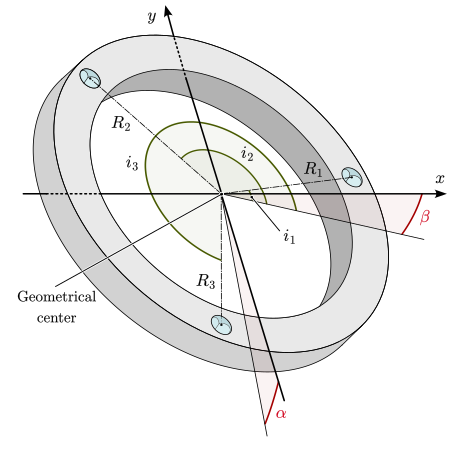
\includegraphics[width=0.7\textwidth]{figures/ring.png}
	\caption{Geometry of the corner cubes on a ring simulating the behaviour of the coil in the real watt balance experiment. Figure taken from \cite[p.11]{Glardon.2024} with slight modifications by the author.}
	\label{fig:ring}
\end{figure}
Let now $I_{OC}(t)$ denote the vertical position of the optical center, and $I_{GC}(t)$ the vertical position of the geometrical center of the corner cubes. Furthermore, $d_x$ and $d_y$ denote the deviations of the optical center from the geometrical center in x- and y-directions in the coil's plane. The angles $\alpha$ and $\beta$ as seen in \cref{fig:ring} are a measure for the tilt angles of the coil around the x-axis ($\alpha$) and around the y-axis ($\beta$). Given these definitions, one can deduce the relation \begin{equation}
	I_{OC}(t) = I_{GC}(t) + \sin[\alpha(t)]d_y - \sin[\beta(t)]d_x
\end{equation} from a consideration of \cref{fig:ring}. Given the geometry of the ring and position measurements $I_1(t)$, $I_2(t)$ and $I_3(t)$ of the vertical position of the three corner cubes on the ring, \cite{5544638} derive the expressions 
\begin{align}
	\begin{aligned}
		\sin[\alpha(t)] = \frac{1}{\det(A)}C_{cos}(t), \quad \sin[\beta(t)] = \frac{1}{\det(A)}C_{sin}(t),
	\end{aligned}
\end{align} where $C_{sin}(t)$ and $C_{cos}(t)$ are defined as \begin{align}\scriptsize
	\begin{aligned}
		C_{cos}(t) &\doteq R_1[I_3(t)-I_2(t)]\cos(i_1) + R_2[I_1(t)-I_3(t)]\cos(i_2)  + R_3[I_2(t)-I_1(t)]\cos(i_3), \\
		C_{sin}(t) &\doteq R_1[I_3(t)-I_2(t)]\sin(i_1) + R_2[I_1(t)-I_3(t)]\sin(i_2) + R_3[I_2(t)-I_1(t)]\sin(i_3).
	\end{aligned}
\end{align} The quantity $\det(A)$ is given entirely by the geometry of the corner cubes on the coil and can be calculated as \begin{equation}
	\det(A) = R_1R_2\sin(i_1-i_2) + R_2R_3\sin(i_2-i_3) + R_3R_1\sin(i_3-i_1).
\end{equation} Furthermore defining \begin{equation}
	C_{GC}(t) \doteq R_1R_3[I_2(t)-I_1(t)]\sin(i_3-i_1) + R_1R_2[I_1(t)-I_3(t)]\sin(i_2-i_1),
\end{equation} the signal $I_{GC}(t)$ specifying the vertical position of the geometrical center is calculated by \begin{equation}
	I_{GC}(t) = I_1(t) + \frac{1}{\det(A)}C_{GC}(t),
\end{equation} as \cite[p.10]{Glardon.2024} states. In total therefore, the reconstructed signal $I_{OC}(t)$ describing the vertical position of the optical center of the coil can be calculated at any time $t$ by \begin{equation}\label{eq:objective_function_dxdy}
	I_{OC}(t) = I_1(t) + \frac{1}{\det(A)}\left[C_{GC}(t) + C_{cos}(t)d_y - C_{sin}(t)d_x\right].
\end{equation}

Fixing the time coordinate $t$ for a certain moment, the above equation thus defined an objective function 
\begin{equation}\label{eq:to_optimize_dxdy}
	\mathcal{L}_{1}(d_x, d_y) = I_1 + \frac{1}{\det(A)}[C_{GC} + C_{cos}d_y - C_{sin}d_x].
\end{equation}
for an optimization process. The parameters to be optimized by this function are $d_x$ and $d_y$, denoting the deviation of the optical center from the geometrical center.

As \cite[p.21-23]{Glardon.2024} shows, there is a bijection between the representation of the position signal $I_{OC}(t)$ as given by \cref{eq:objective_function_dxdy} and a weighted average representation given by \begin{equation}
	I_{OC}(t) = \lambda_1I_1(t) + \lambda_2 I_2(t) + \lambda_3 I_3(t), \quad \sum_{i=1}^{3}\lambda_i = 1.
\end{equation} Given the normalization condition for the weighting parameters, one can also write this equation as \begin{equation}\label{eq:objective_function_weights}
	I_{OC}(t) = \lambda_1 I_1(t) + \lambda_2I_2(t) + (1-\lambda_1-\lambda_2)I_3(t).
\end{equation} This equation defines a second objective function \begin{equation}\label{eq:to_optimize_weights}
	\mathcal{L}_2(\lambda_1,\lambda_2) = \lambda_1 I_1(t) + \lambda_2I_2(t) + (1-\lambda_1-\lambda_2)I_3(t),
\end{equation} which can be optimized by varying $\lambda_1$ and $\lambda_2$ following an optimization goal.

An important observation to state here is that while $\mathcal{L}_1(d_x, d_y)$ requires an a priori assumption for the geometry of the coils corner cubes, $\mathcal{L}_2(\lambda_1,\lambda_2)$ does not. There is however an analytical bijection between both representations, which therefore allows to switch between the $(d_x,d_y)$ and the $(\lambda_1,\lambda_2)$ representations of $I_{OC}(t)$. This means, that the algorithm optimizing $\mathcal{L}_2$ is independent of the geometry of the corner cubes on the coil, while the algorithm optimizing $\mathcal{L}_1$ is not.
% Explain, how the signal is calculated in the optical center

\subsubsection{Optimization routine}
Recalling \cref{eq:verticalpos}, which describes the vertical position $z(t)$ of the optical center and is therefore equivalent to $I_{OC}(t)$, one can state that the optical center is found with regard to \cref{eq:objective_function_dxdy} or \cref{eq:objective_function_weights}, whenever the 1f-term vanishes. This is also to say, that only $2\omega_x$ and $2\omega_y$ will be visible in a frequency spectrum of the signal $I_{OC}(t)$. Alternatively, this also means that the amplitude of the signal $I_{OC}(t)$ is minimized. 

This observation gives rise to two algorithm designs, both implemented and explored by \cite{Glardon.2024}. A first design of the algorithm minimizes the amplitude of the position signal $I_{OC}(t)$ in the optical center, while a second design minimizes the 1f-term peak amplitude as compared to the 2f-term peak amplitude in a frequency spectrum of $I_{OC}(t)$. Furthermore, there are two subdesigns for both types of algorithms, optimizing either the parameters $(d_x, d_y)$ for \cref{eq:to_optimize_dxdy} or $(\lambda_1,\lambda_2)$ for \cref{eq:to_optimize_weights}. As \cite{Glardon.2024} shows in his work, the algorithms minimizing the 1-term peak amplitude as compared to the 2f-term peak amplitude generally performs much better; therefore the work at hand concentrates only on these algorithms. The idea behind such an algorithm is to interatively adapt the parameters $(d_x, d_y)$ or the weights $(\lambda_1, \lambda_2)$, such that the 1f-term peak amplitudes vanish. Note, that the vertical position $I(x,y,t)$ of any coordinates\footnote{The origin of the coordinate system is the geometrical/mechanical center of the coil.} $(x,y)$ in the plane of the coil can be calculated based on \cref{eq:objective_function_dxdy} by \begin{equation}
	I(x,y,t) = I_1(t) + \frac{1}{\det(A)}[C_{GC}(t) + C_{cos}(t)\cdot y - C_{sin}(t)\cdot x]. 
\end{equation} The outcome of an algorithm as described is visualized in \cref{fig:optimization_principle}. The left panels show the reconstructed signals at a position $I(x,y,t)$ in the plane of the coil, whereas the right panels show a section of the respective Fourier transform $\mathcal{F}[I(x,y,t)](\nu)$ obtained by a fast Fourier transform (FFT) algorithm. Hereby, $x$ and $y$ are held constant and only $t$ is Fourier transformed. Clearly, the algorithm optimizing the weights $(\lambda_1, \lambda_2, \lambda_3)$ given \cref{eq:to_optimize_weights} successfully minimizes the 1f peak amplitudes relative to the 2f peak amplitudes.
\begin{figure}[h]
	\centering
	\begin{subfigure}[t]{\textwidth}
		\centering
		\includegraphics[width=\textwidth]{//METASFS01.AD.METAS/HOME$/OFFICE/ZADA/PhD Daniel Zahnd/Joule-watt balance project/Python code/Fourier transform experiments/function_and_fourier_transform_real_data_I_OC_delocated.pdf}
		\caption{Signal of vertical position at point slightly deranged from optical center; $I(d_x+\epsilon_x, d_y + \epsilon_y,t)$. The dominating frequency seem to be the 1f-frequencies $\nu_x = \omega_x(2\pi)^{-1}$ and $\nu_y = \omega_y(2\pi)^{-1}$. Both the 1f- and 2f-signals are superimposed with high-frequency oscillations not seen in the right panel.}
		\label{fig:opticalcenterderanged}
	\end{subfigure}
	\begin{subfigure}[t]{\textwidth}
		\centering
		\includegraphics[width=\textwidth]{//METASFS01.AD.METAS/HOME$/OFFICE/ZADA/PhD Daniel Zahnd/Joule-watt balance project/Python code/Fourier transform experiments/function_and_fourier_transform_real_data_I_OC.pdf}
		\caption{Signal of vertical position at optical center; $I(d_x,d_y,t) = I_{OC}(t)$. The dominating frequencies are the 2f-frequencies $2\nu_x = 2\omega_x(2\pi)^{-1}$ and $2\nu_y = \omega_y(2\pi)^{-1}$. The 2f-signals are superimposed with high-frequency oscillations not seen in the right panel.}
		\label{fig:opticalcenter}
	\end{subfigure}
	\caption{Signals $I(x,y,t)$ describing the vertical position for coordinates $(x,y)$ in the plane of the coil.}
	\label{fig:optimization_principle}
\end{figure}

\subsubsection{PicoScale adjustment procedure}\label{sec:picoscale}
Consider two signals
\begin{equation}
	x(\Delta \phi) = G_x\cos(\Delta \phi + \Delta \phi_{0,x}) + G_{0,x}, \quad y(\Delta \phi) = G_y\sin(\Delta \phi + \Delta \phi_{0,y})  + G_{0,y}
\end{equation}
that form a quadrature signal and hence a so-called Lissajous figure. Hereby, $G_x$ and $G_y$ are the amplitudes for the signals in both x- and y-direction of the coordinate system. Furthermore, $\Delta \phi$ serves as the argument of dependence of the signals $x(\Delta \phi)$ and $y(\Delta \phi)$. Then, there are the parameters $G_{0,x}$, $G_{0,y}$, which are amplitude offsets in both x- and y-directions. Furthermore, one has the parameters $\Delta \phi_{0,x}$ and $\Delta \phi_{0,y}$, which are offsets in the phase difference of both signals. In vectorial notation, one therefore has
\begin{equation}\label{eq:lissajous}
	\boldsymbol{x}(\Delta \phi) = \begin{pmatrix} x(\Delta \phi) \\ y(\Delta \phi) \end{pmatrix} = \begin{pmatrix} G_x \cos(\Delta \phi + \Delta \phi_{0,x}) \\ G_y \sin(\Delta \phi + \Delta \phi_{0,y}) \end{pmatrix} + \boldsymbol{G}_0,
\end{equation}
where $\boldsymbol{G}_0 = (G_{0,x}, G_{0,y})^\top$. If $\boldsymbol{G}_0 = 0$, $G_x = G_y$ and $\Delta \phi_{0,x} = \Delta \phi_{0,y} = 0$, then $\boldsymbol{x}(\Delta \phi)$ describes a so-called perfect Lissajous figure; an exact circle in dependence of $\Delta \phi$ in the x-y-plane. See \cref{fig:perfect_imperfect} for a visualization of an imperfect and perfect Lissajous figure with associated parameter settings.
\begin{figure}[h]
	\centering
	\begin{subfigure}{0.49\textwidth}
		\centering
		\includegraphics[width=\textwidth]{figures/imperfect_liss.pdf}
		\caption{Imperfect Lissajous figure.}
		\label{fig:imperfect_liss}
	\end{subfigure}
	\hfill
	\begin{subfigure}{0.49\textwidth}
		\centering
		\includegraphics[width=\textwidth]{figures/perfect_liss.pdf}
		\caption{Perfect Lissajous figure.}
		\label{fig:perfect_liss}
	\end{subfigure}
	\caption{Imperfect and perfect Lissajous figures with associated parameters with respect to \cref{eq:lissajous}.}
	\label{fig:perfect_imperfect}
\end{figure} In this figure, a whole round-trip around the Lissajous figure corresponds to $\Delta \phi \in [0,\lambda]$ for $\lambda = \SI{1550}{\nano\meter}$ the used wavelength of the laser.

Oftentimes, Michelson-interferometers like that employed by the PicoScale technique, one has two signals $x(\Delta \phi)$ and $y(\Delta \phi)$ in quadrature sent through the interferometer. ``In quadtrature'' hereby means, that $x(\Delta \phi)$ and $y(\Delta \phi)$ ideally employ a $\pi/2$ phase difference, as it is the case with $x(\Delta \phi)$ being proportional to $\cos(\Delta \phi)$ and $y(\Delta \phi)$ being proportional to $\sin(\Delta \phi)$. This technique allows one to be sensitive in the $x$-signal, whenever one is insensitive in the $y$-signal, and vice versa. However, due to misalignment with verticality or horizontality of the target mirror and due to other imperfections in the interferometer setup, the phase difference is never exactly $\pi/2$, nor are the amplitudes $G_x$ and $G_y$ exactly equal, nor are the offsets $G_{x,0}$ and $G_{y,0}$ exactly zero. Therefore, the interferometer setup - like the PicoScale device - auto-adjusts the parameter set $\{G_x, G_y, G_{x,0}, G_{y,0}, \Delta \phi_{0,x}, \Delta \phi_{0,y}\}$ after one manually adjusts the setup with verticality and horinzontality as required; see \cite[p.23]{SmarAct.2019} for more information about this auto-adjustment process.

Depending on the settings of these parameters however, an identical distance might be measured to be equal to different distances, which is why this might result in a problem concerning the reproducibility of length measurements when rebuilding a setup. According to \cite[p.23]{SmarAct.2019}, the PicoScale device establishes a relationship between the vector $\vect{x}(\Delta \phi)$ as given by \cref{eq:lissajous} and the displacement $\Delta s$ of the target mirror as given by the relation \begin{equation}
	\Delta s = \frac{\lambda}{2\pi}\Delta \phi.
\end{equation} If $\vect{x}(\Delta \phi)$ does not describe a perfect Lissajous figure, then the above relation becomes non-linear, which is why distance measurements become erroneous, since they implicitly use the linear relationship as given above.

\subsubsection{Influence of pressure fluctuations on length measurements}
It is the case that a medium changes the index of refraction for light. The index of refraction is commonly denoted by $n$ with an appropriate subscript giving reference to the medium to which it refers. Let $c_{vac}$ denote the speed of light in vacuum and $c_{med}$ the speed of light in a medium. Furthermore, if $\lambda_{vac}$ denotes the wavelength in vacuum, $n_{med}$ the index of refraction in a medium and $\lambda_{med}$ the wavelength in the latter, the defined quantities relate as \begin{equation}
	c_{vac} = n_{med}c_{med}, \qquad \lambda_{med} = \frac{c_{med}}{\nu}, \qquad \lambda_{vac} = \frac{c_{vac}}{\nu},
\end{equation} where $\nu$ refers to the frequency of the light which is invariant in the non-relativistic case across different media. In particular if $n_{med} > 1$ as it is the case for air, the relation \begin{equation}
	\lambda_{med} = \frac{c_{med}}{\nu} < \frac{c_{vac}}{\nu} = \lambda_{vac} = n_{med}\lambda_{med}.
\end{equation} This is to say that if $n_{med} > 1$, then a given wavelength is larger in vacuum than it is in the medium. Concerning length measurements of a length $L_{vac}$, this means that one obtains larger lengths for $L_{vac}$ if it is measured in a medium; then, the relation \begin{equation}\label{eq:conversion_medium_to_vacuum}
	L_{med} = n_{med}L_{vac} \quad \Leftrightarrow \quad L_{vac} = \frac{L_{med}}{n_{med}}
\end{equation} holds for the conversion of measured lengths $L_{med}$ to the corresponding length $L_{vac}$ if it were measured in a vacuum.

The refractive index of air can be calculated using the so-called Edlén equation\footnote{See for example \url{https://emtoolbox.nist.gov/wavelength/Documentation.asp}, link last checked on April 05, 2024.}, which gives the refractive index $n_{air}$ depending on relative humidity $H_R$, temperature $T$, $\textrm{CO}_2$ concentration $X_{\textrm{CO}_2}$ and pressure $P$; therefore, it is a function \begin{equation} 
	n_{air} = n_{air}(T, H_R, \textrm{CO}_2, P).
\end{equation}

\section{Practical implementation of the 3-interferometer technique}
Implementing the 3-interferometer technique to the current METAS Kibble balance setup requires additional time interval analyzers to count the fringes and the associated time intervals between zero-crossings of the interferometer signals. At METAS, an IDQ ID900 time controller\footnote{See \cite{IDQ.2018} for further information.} is available to take over that task. It has however to be studied yet, how this can be achieved. Furthermore, also more than the currently available components such as beam-splitters and optical fibres are necessary.

\subsection{Measurement circuit}
A coarse overview of the measurement circuit for the implementation of the 3-interferometer technique is visualized in \cref{fig:measurement_circuit}.
\begin{figure}[h]
	\centering
	\includegraphics[width=0.65\textwidth]{figures/measurement_circuit.pdf}
	\caption{Overview of the optical circuit for the implementation of the 3-interferometer technique.}
	\label{fig:measurement_circuit}
\end{figure}
The circuit features the PicoScale device used to read out the optical information gathered by the interferometer heads. Furthermore, it features photodetectors used to translate the optical superposition of interferometer signals to a processable output to use as input for the time interval analyzer. The time interval analyzer then records the timestamps of zero-crossings of the interferometer signal for each of the three channels. Knowing the wavelength of the used laser, one can then calculate distances and velocities as indicated and explained with \cref{fig:dataprocessing} and \cref{sec:dataprocessingtheory_v1}.

\subsection{Description of the TIA device}
The time interval analyzer features 4 inputs for an electric signal ranging between $-\SI{3}{\volt}$ and $+\SI{3}{\volt}$. It can be controlled using either the shipped graphical user interface, LabVIEW or \verb|python|; it should be able to get timestamps of zero-crossings of interference signals of an interferometer.

\subsection{Signals to process}
The signals to process by the time interval analyzers are interference signals provided by the photodetectors as seen in \cref{fig:measurement_circuit}. These signals are based on interference patterns as provided by the interferometer heads.

\subsection{Required output}
The required output of the time interval analyzer are the timestamps of zero-crossings for the interferometer signal of each of the three interferometers. Using these timestamps and knowing the wavelength of the used laser light, one can then calculate distances and velocities of the moving mirrors as visualized in \cref{fig:measurement_circuit} and \cref{fig:dataprocessing}.

\subsection{Experiment 1: Providing signal to TIA and getting timestamps}
In order to take the available time interval analyzer into operating mode, a first preliminary experiment was carried out. This experiment consisted of providing a square pulsed signal of frequency $\nu = \SI{840}{\hertz}$ generated by a frequency generator to an input of the time interval analyzer. The time interval analyzer was programmed such that is acquired the timestamps of positive zero-crossings of the signal. The acquired timestamps can then expected to have a spacing of $\Delta t$ matching the provided frequency by means of the relation $\nu = 1/\Delta t$.
\begin{figure}[h]
	\centering
	\includegraphics[width=0.7\textwidth]{figures/freq_prel_exp_scatter.pdf}
	\caption{Outcome for the described experiment. The filled red line denotes the mean value, while the dotted red lines indicate the standard deviation of the acquired dataset.}
	\label{fig:freq_prel_exp_scatter}
\end{figure}
In \cref{fig:freq_prel_exp_scatter}, the results of the described experiment can be seen. 

One can see that the acquired timestamps of the time interval analyzer do lead to plausible values for the frequencies, as the mean value of frequency is $\bar{\nu} = 839.997 \pm \SI{0.017}{\hertz}$, which is in accordance with the set value of $\SI{840}{\hertz}$. In the case at hand, a relative uncertainty of $\sigma_{\bar{\nu}}/\bar{\nu} \approx 2.02\cdot 10^{-5}$ is achieved.

\subsection{Experiment 2: Frequency sweep experiment}
This second experiment consisted of supplying a variable frequency to a time interval analyzer input, whose threshold for making a timestamp was set to a positive flank at about half the peak-to-peak voltage value of the supplied signal. The supplied frequency $\nu$ was set to a linear frequency sweep of $\SI{20}{\second}$ duration in the interval $\nu \in [\SI{100}{\hertz}, \SI{1000}{\hertz}]$. The time interval analyzer recorded the timestamps of positive flanks, wherefrom differences $\Delta t_i$ between timestamps $t_{i+1}$ and $t_i$ could be calculated and hence the associated frequencies $\nu_i = 1/\Delta t_i$. The results of this experiment are given in \cref{fig:freq_sweep_outcomes}.
\begin{figure}[h]
	\centering
	\begin{subfigure}[t]{0.49\textwidth}
	\centering
	\includegraphics[width=\textwidth]{figures/freq_lin_sweep.pdf}
	\caption{Results for the frequency $\nu$.}
	\label{fig:freq_lin_sweep}
	\end{subfigure}
	\hfill
	\begin{subfigure}[t]{0.49\textwidth}
	\centering
	\includegraphics[width=\textwidth]{figures/vel_lin_sweep.pdf}
	\caption{Results for the velocity $v$.}
	\label{fig:vel_lin_sweep}
	\end{subfigure}
	\caption{Frequency sweep experiment outcome.}
	\label{fig:freq_sweep_outcomes}
\end{figure}
Note, that \cref{fig:freq_sweep_outcomes} shows the calculated velocity $v$, if the provided signal to the time interval analyzer is assumed to be an interferometer signal, where the interferometer is assumed to have a wavelength of $\lambda = \SI{1550}{\nano\meter}$.

The obtained results indicate, that the time interval analyzer indeed does what it should do and furthermore show, that a signal of expected frequency around $\SI{840}{\hertz}$ can be accurately processed by the TIA. Thus one can conclude, that the TIA works well for square signal frequencies in the range $\nu \in [\SI{100}{\hertz}, \SI{1000}{\hertz}]$.
\subsection{Experiment 3: Frequency stability experiment}
This third experiment consisted of supplying to the time interval analyzer input a constant frequency of $\SI{840}{\hertz}$ over a time window of 300 seconds. The goal of this experiment was to determine the discrimination stability of the time interval analyzer input, assuming that the signal generated by the frequency generator has negligible noise. The obtained timestamps by the TIA were converted to frequencies; the results can be seen in \cref{fig:freq_stab_exp_scatter}.
\begin{figure}[h]
	\centering
	\includegraphics[width=0.7\textwidth]{figures/freq_stab_exp_scatter.png}
	\caption{Frequency stability experiment outcome. The filled red line denotes the mean value, while the dotted red lines indicate the standard deviation of the acquired dataset.}
	\label{fig:freq_stab_exp_scatter}
\end{figure}

If one denotes the standard deviation of the dataset by $\sigma_{\bar{\nu}}$, one can conclude that most of the datapoints are indeed within a $2\sigma_{bar{\nu}}$ range around the mean value $\bar{\nu}$, thus indicating that the noise is Gaussian in nature. One can also perceive, that the frequency does seem to fluctuate around a constant value of $\bar{\nu}$; however, a slight tendency of the noise to increase with time can be perceived. In the prevalent case, a relative uncertainty of $\sigma_{\bar{\nu}}/\bar{\nu} \approx 1.79\cdot 10^{-5}$ is obtained.

\chapter{Joule balance}
\section{Introduction}
The joule balance as proposed and implemented by \cite{Xu_2016} is actually a generalized concept of the Kibble balance principle. Depending on the nature of Kibble balance implementation, one can use a Kibble balance as a joule balance with comparatively little additional modifications. 

Simply put, mechanical and electrical virtual power are compared only at a fixed vertical position of the balance in the Kibble balance experiment. The joule balance experiment however equates the time integrals of mechanical and electrical virtual power and hence relates electrical to mechanical virtual energy; thus the name ``joule balance''.

%A Kibble balance, also known as watt balance, requires two phases of measurement; a dynamic phase and a static phase. In the static phase of the Kibble balance, a so-called weighing of the mass is performed at a fixed vertical position of the balance. In the static phase, a weight is placed on the mass pan of the balance, whose gravitational force is then balanced by a generated electromagnetic force. This force is generated by injecting a current into a coil placed inside a static magnetic field, the former being attached to the mass pan. The measured quantity in this phase is the current required to balance the weight in the Kibble balance. The dynamic phase then moves the coil up and down with a certain velocity profile. Since moving a conductor in a magnetic field generates a voltage, the induced voltage in the coil is the measured quantity in this case. Voltage times current equals a electrical power, whereas force times velocity gives a mechanical power. The 

\section{General principle}
The general working principle of the joule balance is very similar to that of the Kibble balance. One can start from the fundamental general equation 
\begin{equation}\label{eq:joulebalancestart}
	\overbrace{\underbrace{\vect{F}(\vect{r},t)\cdot \vect{v}(t)}_{\text{Translational power}} + \underbrace{\vect{M}(\vect{r},t)\cdot \vect{\omega}(t)}_{\text{Rotational power}}}^\text{Total mechanical power} = \underbrace{I(t) U(t)}_{\text{Electrical power}}
\end{equation}
governing the Kibble balance, which was derived in \cref{sec:deriv_Kibble_balance}. Hereby, $\vect{F}(\vect{r},t)$ is the force acting on the balance at position $\vect{r}$, $\vect{v}(t)$ is the velocity with which the coil is moved in the dynamic phase using a linear actuator, $\vect{M}(\vect{r},t)$ is a torque exerted on the coil due to misalignments $\vect{\omega}(t)$ is the associated angular velocity to the torque, $I(t)$ is the current injected in the static phase to balance the gravitational force of the test mass and $U(t)$ is the induced voltage in the coil in the dynamic phase.

Now, note that $\vect{v}(t) = \frac{\mathrm{d}\vect{r}(t)}{\mathrm{d}t}$ and that $\vect{\omega}(t) = \frac{\mathrm{d}\vect{\theta}(t)}{\mathrm{d}t}$, where $\vect{r}(t)$ is the position of the center of mass of the coil and $\vect{\theta}(t)$ is the angular displacement of the coil's fixed coordinate system to a rest coordinate system. Let furthermore $t_1$ be the time at which the balance is at its lower position of the dynamic phase and $t_2$ the time at which the balance is at its upper position. Let furthermore $\vect{r}(t_1) = (x(t_1), y(t_1), z(t_1))^\top \doteq (x_1, y_1, z_1)^\top \doteq \vect{r}_1$ and $\vect{r}(t_2) = (x(t_2), y(t_2), z(t_2))^\top \doteq (x_2, y_2, z_2)^\top \doteq \vect{r}_2$ be the associated position coordinates of the center of mass of the coil at times $t_1$ and $t_2$; the associated angular deviations are similarly given as $\vect{\theta}(t_1) = (\theta_x(t_1), \theta_y(t_1), \theta_z(t_1))^\top \doteq (\theta_{x1}, \theta_{y1}, \theta_{z1})^\top \doteq \vect{\theta}_1$ and  $\vect{\theta}(t_2) = (\theta_x(t_2), \theta_y(t_2), \theta_z(t_2))^\top \doteq (\theta_{x2}, \theta_{y2}, \theta_{z2})^\top \doteq \vect{\theta}_2$.

Using these definitions, one can integrate \cref{eq:joulebalancestart} with respect to time $t$ from $t_1$ to $t_2$, such that one obtains \begin{equation}
	\int_{\vect{r}(t_1)}^{\vect{r}(t_2)}\frac{\vect{F}(\vect{r},t)}{I(t)}\cdot \frac{\mathrm{d}\vect{r}(t)}{\mathrm{d}t}\,\mathrm{d}t + \int_{\vect{\theta}(t_1)}^{\vect{\theta}(t_2)}\frac{\vect{M}(\vect{r},t)}{I(t)}\cdot \frac{\mathrm{d}\vect{\theta}(t)}{\mathrm{d}t}\,\mathrm{d}t = \int_{t_1}^{t_2}U(t)\,\mathrm{d}t.
\end{equation} Simplifying this expression leads to the equation \begin{equation}
\int_{\vect{r}_1}^{\vect{r}_2}\frac{\vect{F}(\vect{r})}{I(\vect{r})}\cdot \mathrm{d}\vect{r} + \int_{\vect{\theta}_1}^{\vect{\theta}_2}\frac{\vect{M}(\vect{\theta})}{I(\vect{\theta})}\cdot \mathrm{d}\vect{\theta} = \int_{t_1}^{t_2}U(t)\,\mathrm{d}t.
\end{equation} 

The goal of the alignment procedure of any joule balance would be, that the second integral and all but the z-component of the first integral of the above equation vanish; and that the current $I(\vect{r})$ does only depend on where the weighting was performed on the z-axis, thus $I(\vect{r}) = I(z)$. Also, the force measurements are performed along the z-axis, therefore one can write $\vect{F}(\vect{r}) = \vect{F}(z)$. Provided that the x- and y-component integrals of the force along the trajectory $\vect{r}(t)$ of the coil integrate to zero, the equation \begin{equation}\label{eq:joule_first_int_equation}
	\int_{z_1}^{z_2} \frac{F_z(z)}{I(z)}\,\mathrm{d}z = m\int_{z_1}^{z_2} \frac{g(z)}{I(z)}\,\mathrm{d}z = \int_{t_1}^{t_2}U(t)\,\mathrm{d}t.
\end{equation} thus results, where it was used in a second step that the vertical force $F_z(z)$ is given by the gravitational acceleration $g(z)$ times the mass $m$ of the weighted object.

Given that the current $I(z)$ is measured at each position $z$ using a digital voltmeter calibrated against a Josephson voltage standard and a resistor calibrated against a quantum Hall resistance standard, one can by similarity to \cref{eq:quantum_josephson} write \begin{equation}\label{eq:joule_current}
	I(z) = C_I(z)\frac{n_{J,I}(z)f_{J,I}(z)n_H e}{2},
\end{equation} where $C_I(z)$ is a calibration constant, $n_{J,I}(z)$ is an integer number of Josephson junctions used for the measurement at position $z$, $f_{J,I}(z)$ is the Josephson frequency used for the measurement at position $z$, $n_H$ is an integer number quantifying the quantum Hall resistance and $e$ is the elementary charge. Similarly, given that $U(t)$ is measured at each time $t(z)$ using a voltmeter calibrated against a Josephson voltage standard, one can formulate the equation \begin{equation}\label{eq:joule_voltage}
U(t) = C_U(t)\frac{h}{2e}n_{J,U}(t)f_{J,U}(t).
\end{equation} Here, $C_U(t)$ is a calibration constant, $n_{J,U}(t)$ is an integer number of Josephson junctions used for the measurement at time $t(z)$ and $f_{J,I}(t)$ is the Josephson frequency used for the measurement at time $t(z)$. Defining the new calibration constants \begin{equation}
\tilde{C}_I(z) \doteq \frac{2}{C_I(z)n_{J,I}(z)n_H}, \qquad \tilde{C}_U(t) \doteq \frac{C_U(t)n_{J,U}(t)}{2},
\end{equation} and inserting these expressions along with \cref{eq:joule_current} and \cref{eq:joule_voltage} into \cref{eq:joule_first_int_equation}, one obtains the integral equation \begin{equation}
m\int_{z_1}^{z_2}\tilde{C}_I(z)\frac{g(z)}{f_{J,I}(z)}\,\mathrm{d}z = h \int_{t_1}^{t_2}\tilde{C}_U(t)f_{J,U}(t)\,\mathrm{d}t
\end{equation} relating the mass $m$ to the Planck constant $h$ by means of the measured quantities $g(z)$, $\tilde{C}_I(z)$, $f_{J,I}(z)$, $\tilde{C}_U(t)$ and $f_{J,U}(t)$. The final equation in the form ``mass equals Planck constant times measured quantities'' can be obtained by means of rearranging; finally, the fundamental joule balance equation \begin{equation}\label{eq:fundamental_joule_balance_equation}
m = h\left(\int_{z_1}^{z_2}\tilde{C}_I(z)\frac{g(z)}{f_{J,I}(z)}\,\mathrm{d}z\right)^{-1}\int_{t_1}^{t_2}\tilde{C}_U(t)f_{J,U}(t)\,\mathrm{d}t
\end{equation} results.


%Using $\vect{F} = (F_x, F_y, F_z)^\top$ and $\vect{M} = (M_x, M_y, M_z)^\top$, one can also write \begin{equation}
%\int_{z_1}^{z_2}F_z\,\mathrm{d}z + \underbrace{\sum_{j \in \{x,y\}} \int_{j_1}^{j_2}F_j\,\mathrm{d}j + \sum_{j \in \{x,y,z\}} \int_{j_1}^{j_2}M_j\,\mathrm{d}\theta_j}_{\text{Parasitic terms}} = \int_{t_1}^{t_2}U(t)\,\mathrm{d}t.
%\end{equation} The parasitic terms are to be minimized 
	
%	\chapter{Literature review}
%	\section{Measurement of the position and
%		velocity of translation of a coil in a
%		magnetic field - Glardon}
%	Using the conventional setup of the corner cube it is difficult to align the experimental setup such that the optical center coincides with the geometrical/mechanical center of the coil. The optical center hereby is the projection of the center of mass down onto the plane of the coil, which is often found to be slightly tilted in reality. This alignment is necessary to infer the vertical velocity of the coil in the dynamic mode. An alternative approach using three corner cubes in the plane of the coil circumvents this problem by inferring the optical center from simultaneous measurements pertaining to the three corner cubes. From that one can then also calculate the estimated vertical position of the optical center $I_{OC}$ as a function of time, as it seems; which is what is necessary to determine the velocity of the coil in dynamic mode.
%	
%	\section{Design of the new METAS watt balance
%		experiment Mark II - Baumann et al.}
%	Text. $\si{\micro\meter}$
%	
%	\section{In situ correction of Abbe offset error in the Watt balance experiment - Haddad et al.}
%	Text.

\appendix
\chapter{Statistics}
\section{Random variable}
A random variable is some quantity $x$, which can take a random value. Those random values follow a certain probability distribution, which is determined by the underlying process constituting the random variable.If the probability distribution of a random variable is known, the probability density $p(x)$ can be written down for the continuous and discrete cases as \begin{equation}
	\int_{-\infty}^{\infty}p(x)\,\mathrm{d}x = 1 \qquad \text{and} \qquad \sum_{i} p(x_i) = 1.
	\end{equation}

\section{Expectation value}
The expectation value $E(x) \doteq \bar{x}$ of a random variable $x$ for both the continuous and discrete case is defined as \begin{equation}
	E(x) = \int_{-\infty}^{\infty}xp(x)\,\mathrm{d}x \qquad \text{and} \qquad E(x) = \sum_{i}x_ip(x_i).
\end{equation}

\section{Variance, standard deviation and covariance}
The variance $V(x)$ of a continuous or discrete random variable $x$ can be calculated by means of \begin{equation}
	V(x) = \int_{-\infty}^{\infty} (x-\bar{x})^2\,\mathrm{d}x \qquad \text{and} \qquad V(x) = \sum_{i} (x_i-\bar{x})^2p(x_i).
\end{equation}
The standard deviation $\sigma_x$ is defined as the square root of the variance, hence \begin{equation}
	\sigma_x = \sqrt{V(x)}.
\end{equation}
Let now $x_1,\dots,x_n$ be random variables with associated probability densities $p(x_j)$, $j\in \{1,\dots,n\}$ and joint probability densities $p(x_i,x_j)$. Let furthermore be $\bar{x}_i = E(x_i)$. The covariance $K(x_i,x_j)$ of two random variables for the continuous and discrete case is defined as \begin{equation}\label{eq:covariance}
	K(x_i,x_j) = \int_{-\infty}^{\infty}\int_{-\infty}^{\infty}(x_i-\mu_i)(x_j-\mu_j)p(x_i,x_j)\,\mathrm{d}x_i\,\mathrm{d}x_j
\end{equation} and \begin{equation}
K(x_i,x_j) = \sum_{k,l}(x_{i_k}-\mu_{i})(x_{j_l}-\mu_j)p(x_{i_k},x_{j_l}).
\end{equation} In the context of covariance, one usually also defines the correlation coefficient $\rho(x_i,x_j)$ between two random variables as \begin{equation}\label{eq:correlationcoefficient}
\rho(x_i,x_j) = \frac{K(x_i,x_j)}{\sqrt{V(x_i)V(x_j)}} = \frac{K(x_i,x_j)}{\sigma_{x_i}\sigma_{x_j}}.
\end{equation} If one has two discrete random variables $a$ and $b$ following a uniform distribution and samples $\{a_1,\dots,a_n\}$ and $\{b_1,\dots,b_n\}$ with $n\in \mathbb{N}$, one can calculate an estimate $s(a,b)$ of the covariance $K(a,b)$ as \begin{equation}
s(a,b) = \frac{1}{n-1}\sum_{i=1}^{n} (a_i-\bar{a})(b_i-\bar{b}).
\end{equation}

\section{Propagation of uncertainties}
Consider some random variables $x_1,\dots,x_n$ and a function $f(x_1,\dots,x_n)$ relating those variables. Let furthermore $\sigma_{x_i}$ be the uncertainties (standard deviations) of the random variables $x_i$ and let $\sigma_{x_ix_j} = \sqrt{K(x_i,x_j)}$ be the joint uncertainties of $x_i$ and $x_j$. In this case, the general propagation of uncertainties $\sigma(x_i)$ on the outcome $f(x_1,\dots,x_n)$ is quantified by the uncertainty $\sigma_f$ as \begin{equation}\label{eq:generallawpropagationofuncertainties}
	\sigma_f = \sqrt{\sum_{i=1}^{n}\left(\frac{\partial f}{\partial x_i}\right)^2 \sigma_{x_i}^2+ 2\sum_{1\leq i<j\leq n}\left(\frac{\partial f}{\partial x_i}\right)\left(\frac{\partial f}{\partial x_j}\right)\sigma_{x_ix_j}^2}.
\end{equation}

\subsection{Application: Uncertainty of correlated methods to determine the same quantity}
Consider two random variables $m_1$ and $m_2$ representing two methods to determine the same quantity $m$. The variable $m_1$ could for example denote the Kibble balance method and $m_2$ the joule balance method to determine the weight of the same mass $m$. The uncertainties associated to both methods shall be denoted by $\sigma_{m_1}$ and $\sigma_{m_2}$; and the correlation coefficient shall be identified with $\rho(m_1,m_2)$.

The quantity $m$ can then be calculated as a weighted average from both methods, namely by \begin{equation}\label{eq:twomethodssamequantity}
	m(m_1,m_2,w_1,w_2) = w_1m_1 + w_2m_2, \qquad w_1 + w_2 = 1,
\end{equation} where $w_1$ and $w_2$ are chosen such that the uncertainty associated with $m$ denoted as $\sigma_m$ is minimized. One can write down an expression for that uncertainty by means of applying the uncertainty propagation law \cref{eq:generallawpropagationofuncertainties} to \cref{eq:twomethodssamequantity}, which amounts to \begin{align}
\begin{aligned}
	\sigma_m &= \left(\sum_{i=1}^{2}\left(\frac{\partial m}{\partial m_i}\right)^2\sigma_{m_i}^2 + 2\sum_{1\leq i<j\leq 2}\left(\frac{\partial m}{\partial m_i}\right)\left(\frac{\partial m}{\partial m_j}\right)\sigma_{m_im_j}^2\right)^{1/2} \\
	&= \left(w_1^2\sigma_{m_1}^2 + w_2^2\sigma_{m_2}^2 + 2w_1w_2\sigma_{m_1m_2}^2\right)^{1/2} \\
	&= \sqrt{w_1^2\sigma_{m_1}^2+w_2^2\sigma_{m_2}^2 + 2w_1w_2\rho(m_1,m_2)\sigma_{m_1}\sigma_{m_2}} \\
	&= \sqrt{w_1^2\sigma_1^2 + w_2\sigma_2^2 +2w_1w_2\rho_{12} \sigma_1\sigma_2},
\end{aligned}
\end{align} where in the last step straightforward short-hand notation was introduced. Choosing the weights $w_1$ and $w_2$ such that the uncertainty of $m$ is minimized means that the function $\gamma(w_1,w_2) \doteq \sigma(m)^2 = \gamma(w_1,1-w_1) = \gamma(w_1)$ given by \begin{equation}
 \gamma(w_1) = w_1^2\sigma_1^2 + (1-w_1)^2\sigma_2^2 + 2w_1(1-w_1)\rho_{12}\sigma_1\sigma_2
\end{equation} is minimized with respect to $w_1$. This leads to the weights \begin{equation}
w_1 = \frac{\sigma_2^2 - \rho_{12}\sigma_1\sigma_2}{\sigma_1^2+ \sigma_2^2 - 2\rho_{12}\sigma_1\sigma_2}, \qquad w_2 = \frac{\sigma_1^2-\rho_{12}\sigma_1\sigma_2}{\sigma_1^2+ \sigma_2^2 + 2\rho_{12}\sigma_1\sigma_2}.
\end{equation} Inserting these weights into the expression for $\sigma_m$, one obtains after tedious term rearrangements \begin{equation}\label{eq:combined_uncertainty}
\sigma_m(\rho_{12}) = \sqrt{\frac{\sigma_1^2\sigma_2^2(1-\rho_{12}^2)}{\sigma_1^2+\sigma_2^2-2\rho_{12}\sigma_1\sigma_2}}.
\end{equation} One can show by standard analysis procedures, that $\rho_m(\rho_{12})$ has a maximum at $\rho_{12} = \sigma_1/\sigma_2$, if $\sigma_1 \leq \sigma_2$ or at $\rho_{12}= \sigma_2/\sigma_1$, if $\sigma_2 \leq \sigma_1$. The corresponding values of the uncertainty $\sigma_m$ on $m$ are \begin{equation}
\sigma_m(\rho_{12}=\sigma_1/\sigma_2) = \sigma_1 \quad \text{if} \quad \sigma_1 \leq \sigma_2
\end{equation} and \begin{equation} \sigma_m(\rho_{12}=\sigma_2/\sigma_1) = \sigma_2 \quad \text{if} \quad \sigma_2  \leq \sigma_1.
\end{equation} From this, one can hence conclude \begin{equation}
\sigma_m(\rho_{12}) \leq \min(\sigma_1,\sigma_2)
\end{equation} for all $\rho_{12} \in [-1,1]$, namely the definition range of the correlation coefficient $\rho_{12}$. If one therefore has two methods $m_1$ and $m_2$ to determine the same quantity $m = w_1m_1 + w_2m_2$, the uncertainty on the outcome $m$ will always be smaller than or equal as the smaller uncertainty of both methods.

An example plot of \cref{eq:combined_uncertainty} for $\sigma_{m_1} = \sigma_1 = 1$ and $\sigma_{m_2} = \sigma_2 = 2$ can be seen in \cref{fig:correlated_procedures}.
\begin{figure}[h]
	\centering
	\includegraphics[width=0.6\textwidth]{figures/correlated_procedures.pdf}
	\caption{Example plot of the combined uncertainty on a quantity $m$ determined by two correlated procedures $m_1$ and $m_2$ by means of $m = w_1m_1 + w_2m_2$, where $w_1$ and $w_2$ are weights $w_1 + w_2 = 1$.}
	\label{fig:correlated_procedures}
\end{figure}
It can be seen from the plot, that indeed the combined uncertainty is always smaller than or equal to the smaller of both input uncertainties $\sigma_1$ or $\sigma_2$; in the case at hand, $\sigma_m \leq \sigma_1$, because $\sigma_1 < \sigma_2$.
	
\bibliography{references}
\bibliographystyle{apalike}
	
\end{document}
